% Appendix Template

\chapter{Dynamic Light Scattering} % Main appendix title

\label{AppendixD} % Change X to a consecutive letter; for referencing this appendix elsewhere, use \ref{AppendixX}
\begin{figure} [ht!]
\centering
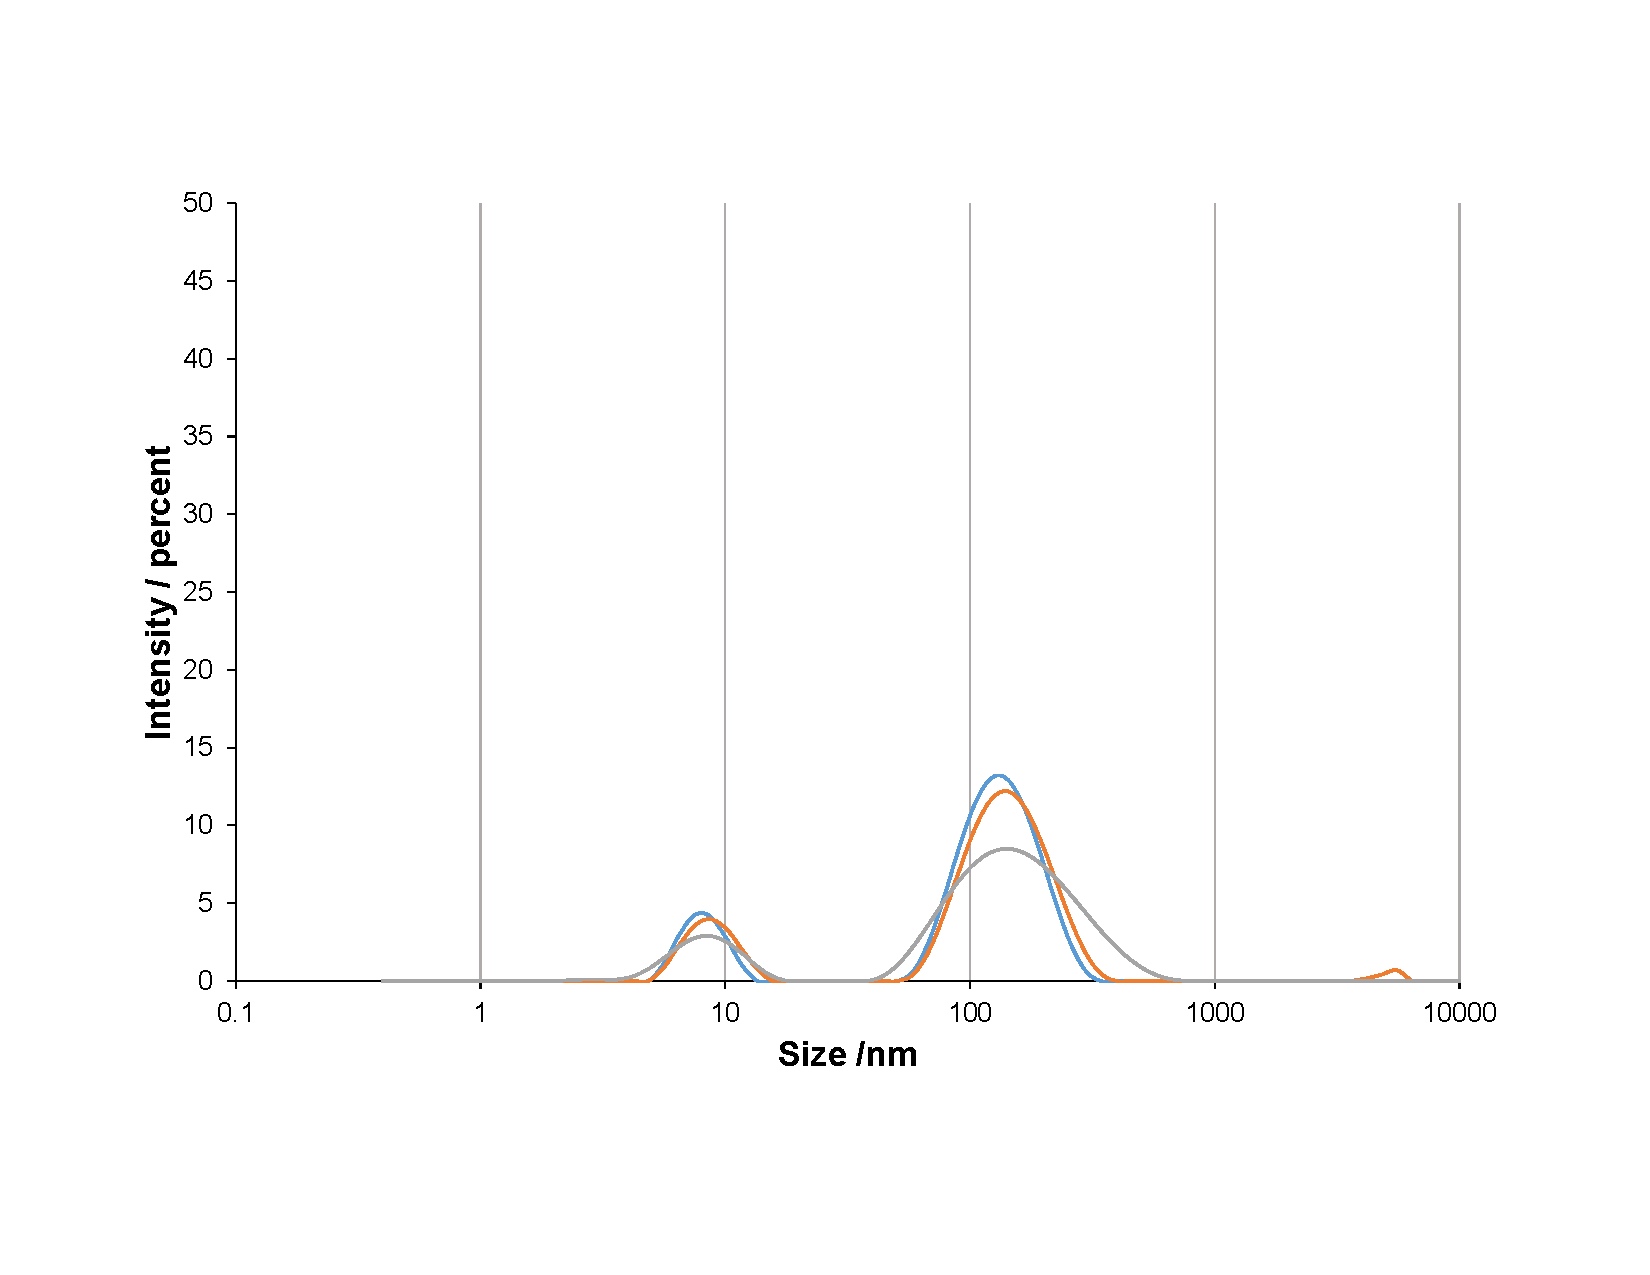
\includegraphics[scale=0.47]{DLS/KAT1_35_0_25mg_ml-1_size.pdf}
\caption{Intensity distribution of a 0.25 mg ml\textsuperscript{-1} sample of C\textsubscript{16}-D-Ala-D-Lys}
\label{intensity_0.25_KAT1.35}
\end{figure}

\begin{figure} [ht!]
\centering
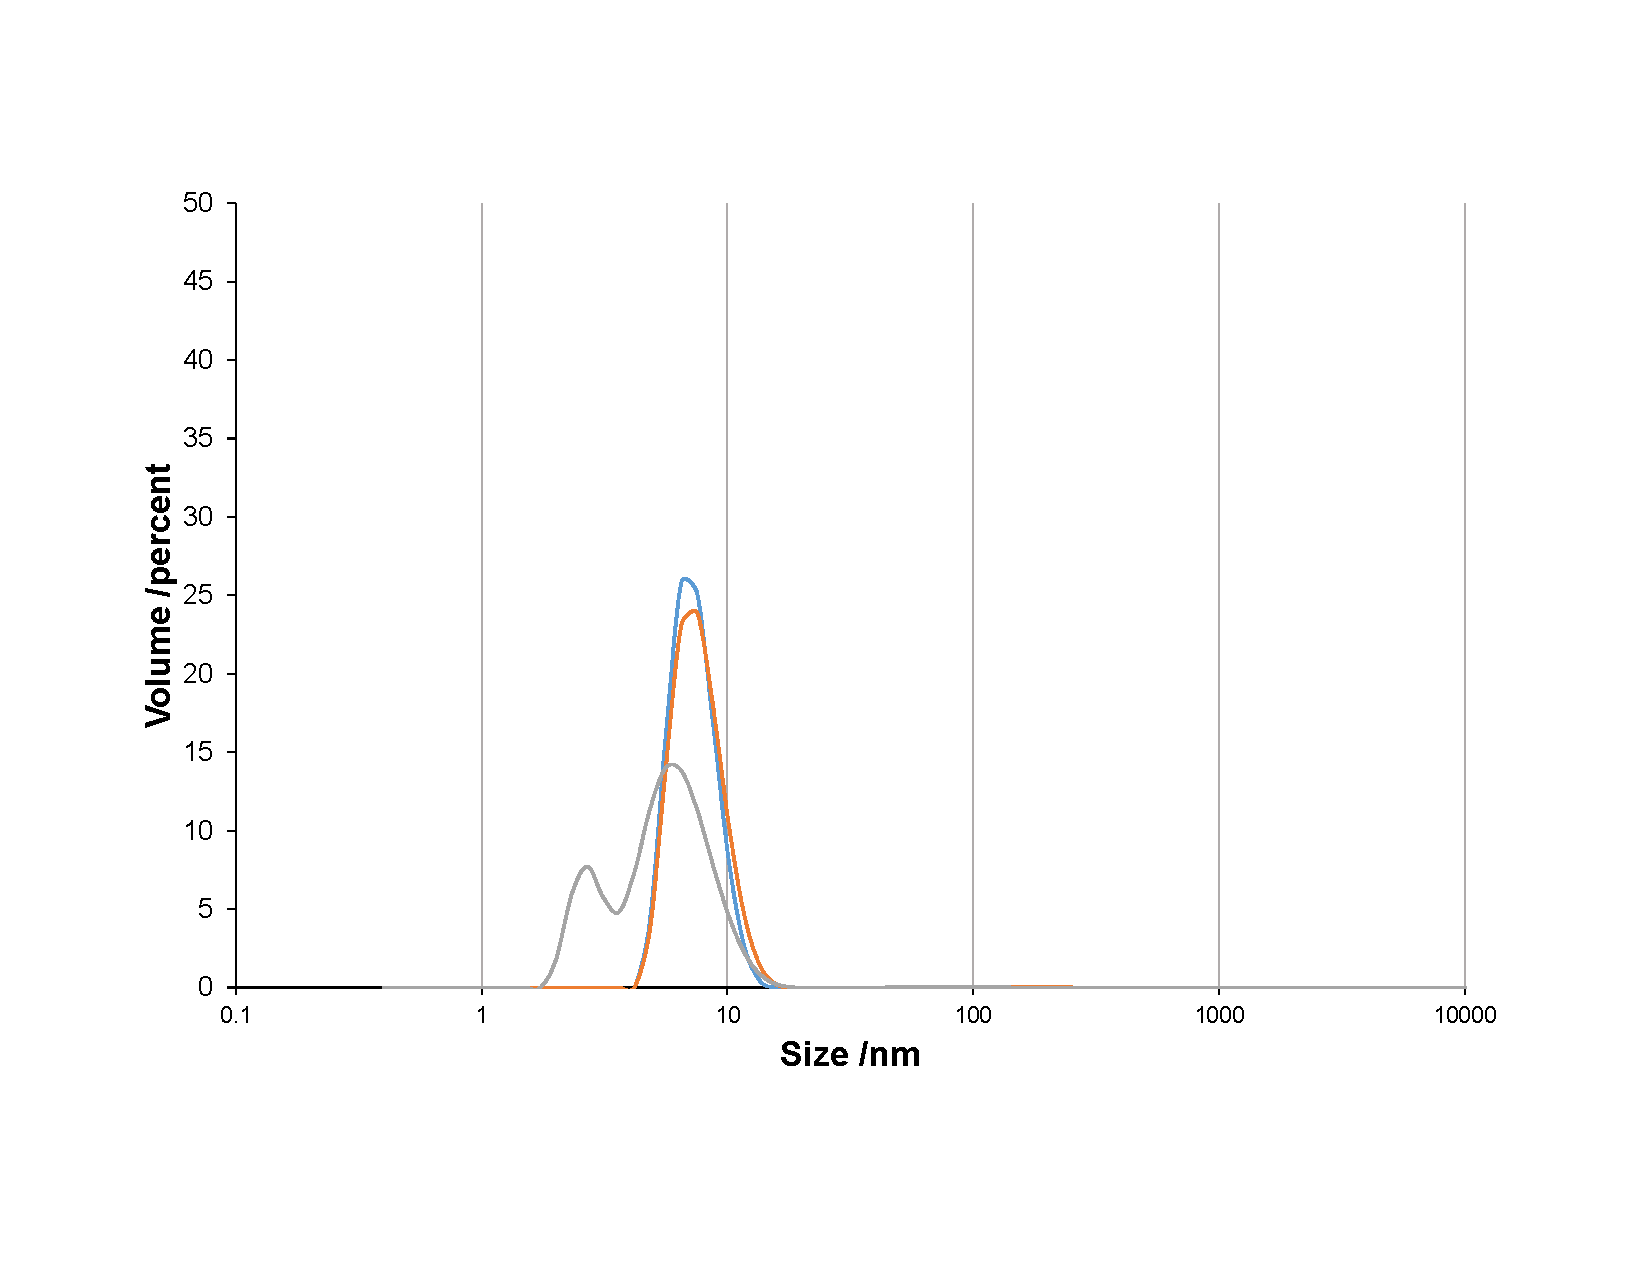
\includegraphics[scale=0.47]{DLS/KAT1_35_0_25mg_ml-1_volume.pdf}
\caption{Volume distribution of a 0.25 mg ml\textsuperscript{-1} sample of C\textsubscript{16}-D-Ala-D-Lys}
\label{volume_0.25_KAT1.35}
\end{figure}

\begin{figure} [ht!]
\centering
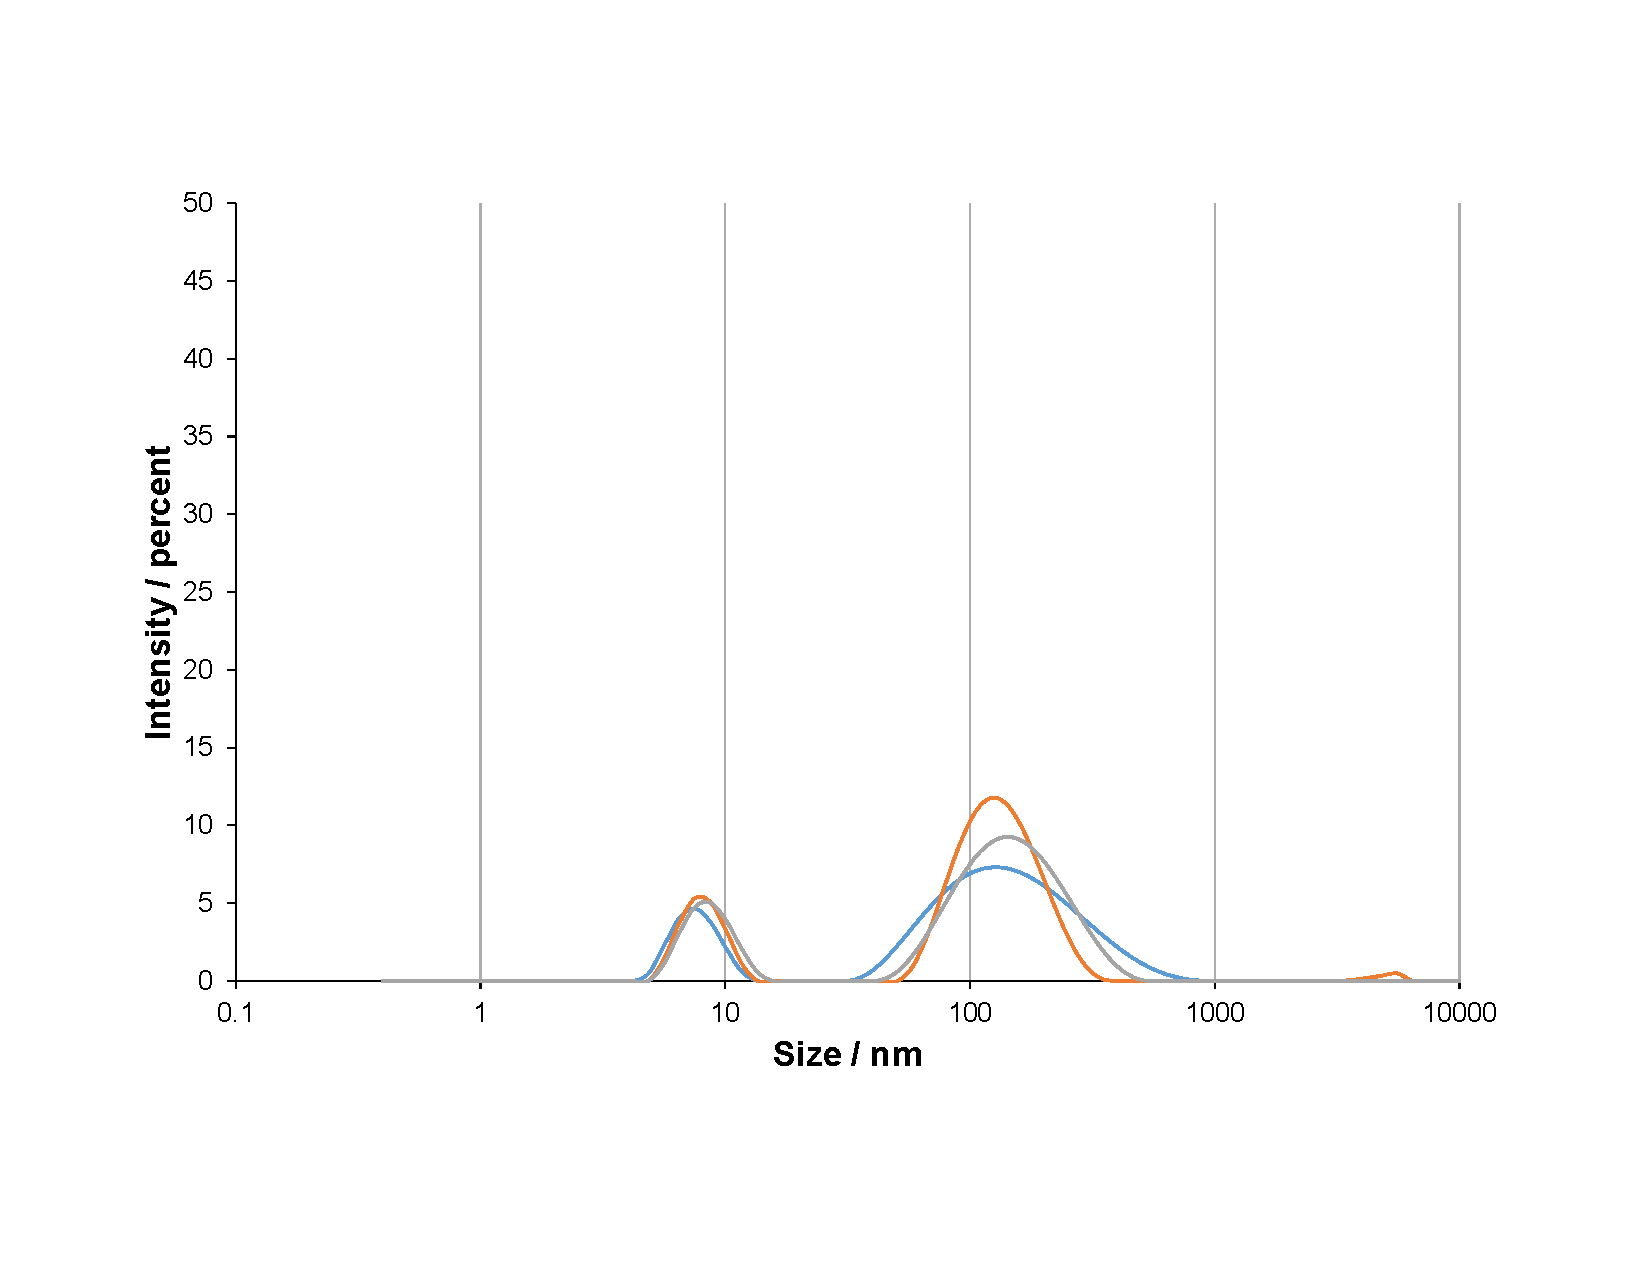
\includegraphics[scale=0.47]{DLS/KAT1_35_1_0mg_ml-1_size.pdf}
\caption{intensity distribution of a 1 mg ml\textsuperscript{-1} sample of C\textsubscript{16}-D-Ala-D-Lys}
\label{intensity_1.0_KAT1.35}
\end{figure}

\begin{figure} [ht!]
\centering
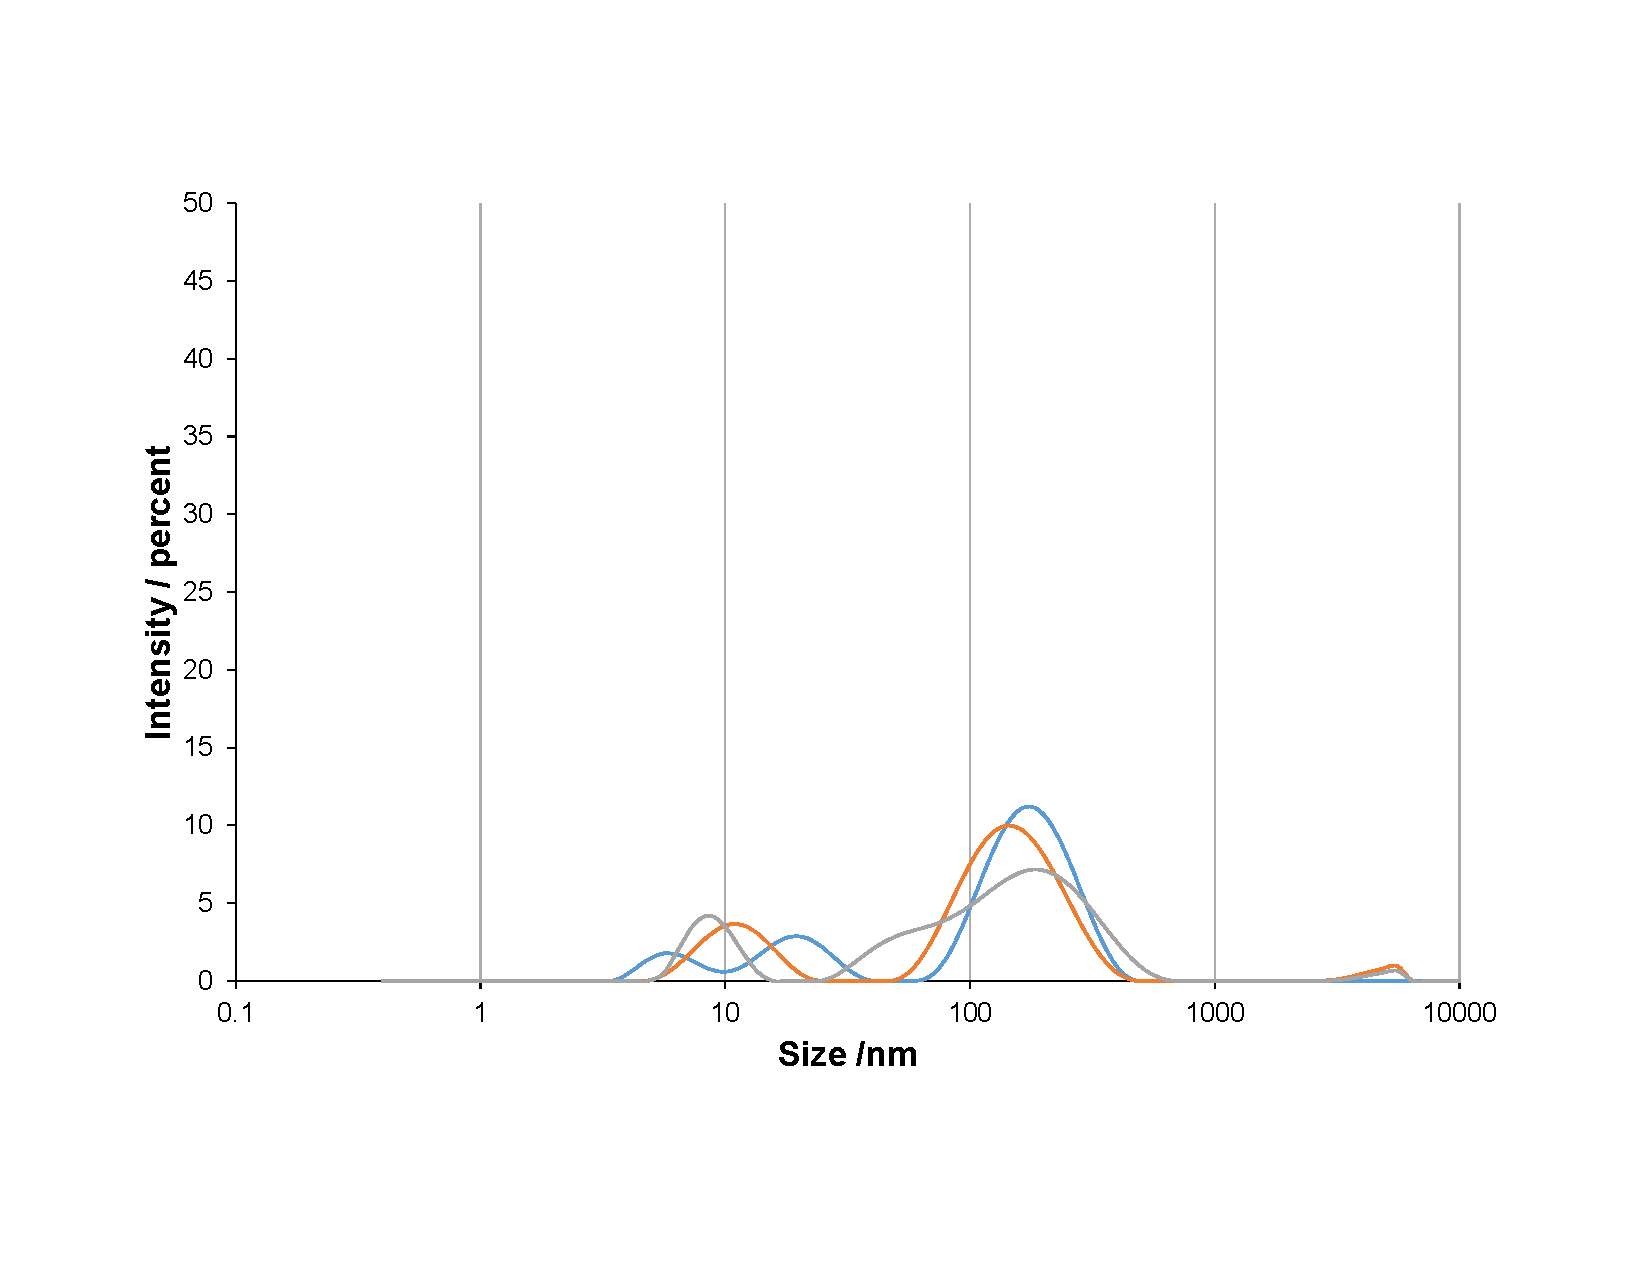
\includegraphics[scale=0.47]{DLS/KAT1_19_0_25mg_ml-1_size.pdf}
\caption{Intensity distribution of a 0.25 mg ml\textsuperscript{-1} sample of C\textsubscript{16}-L-Ala-L-Lys}
\label{intensity_0.25_KAT1.19}
\end{figure}

\begin{figure} [ht!]
\centering
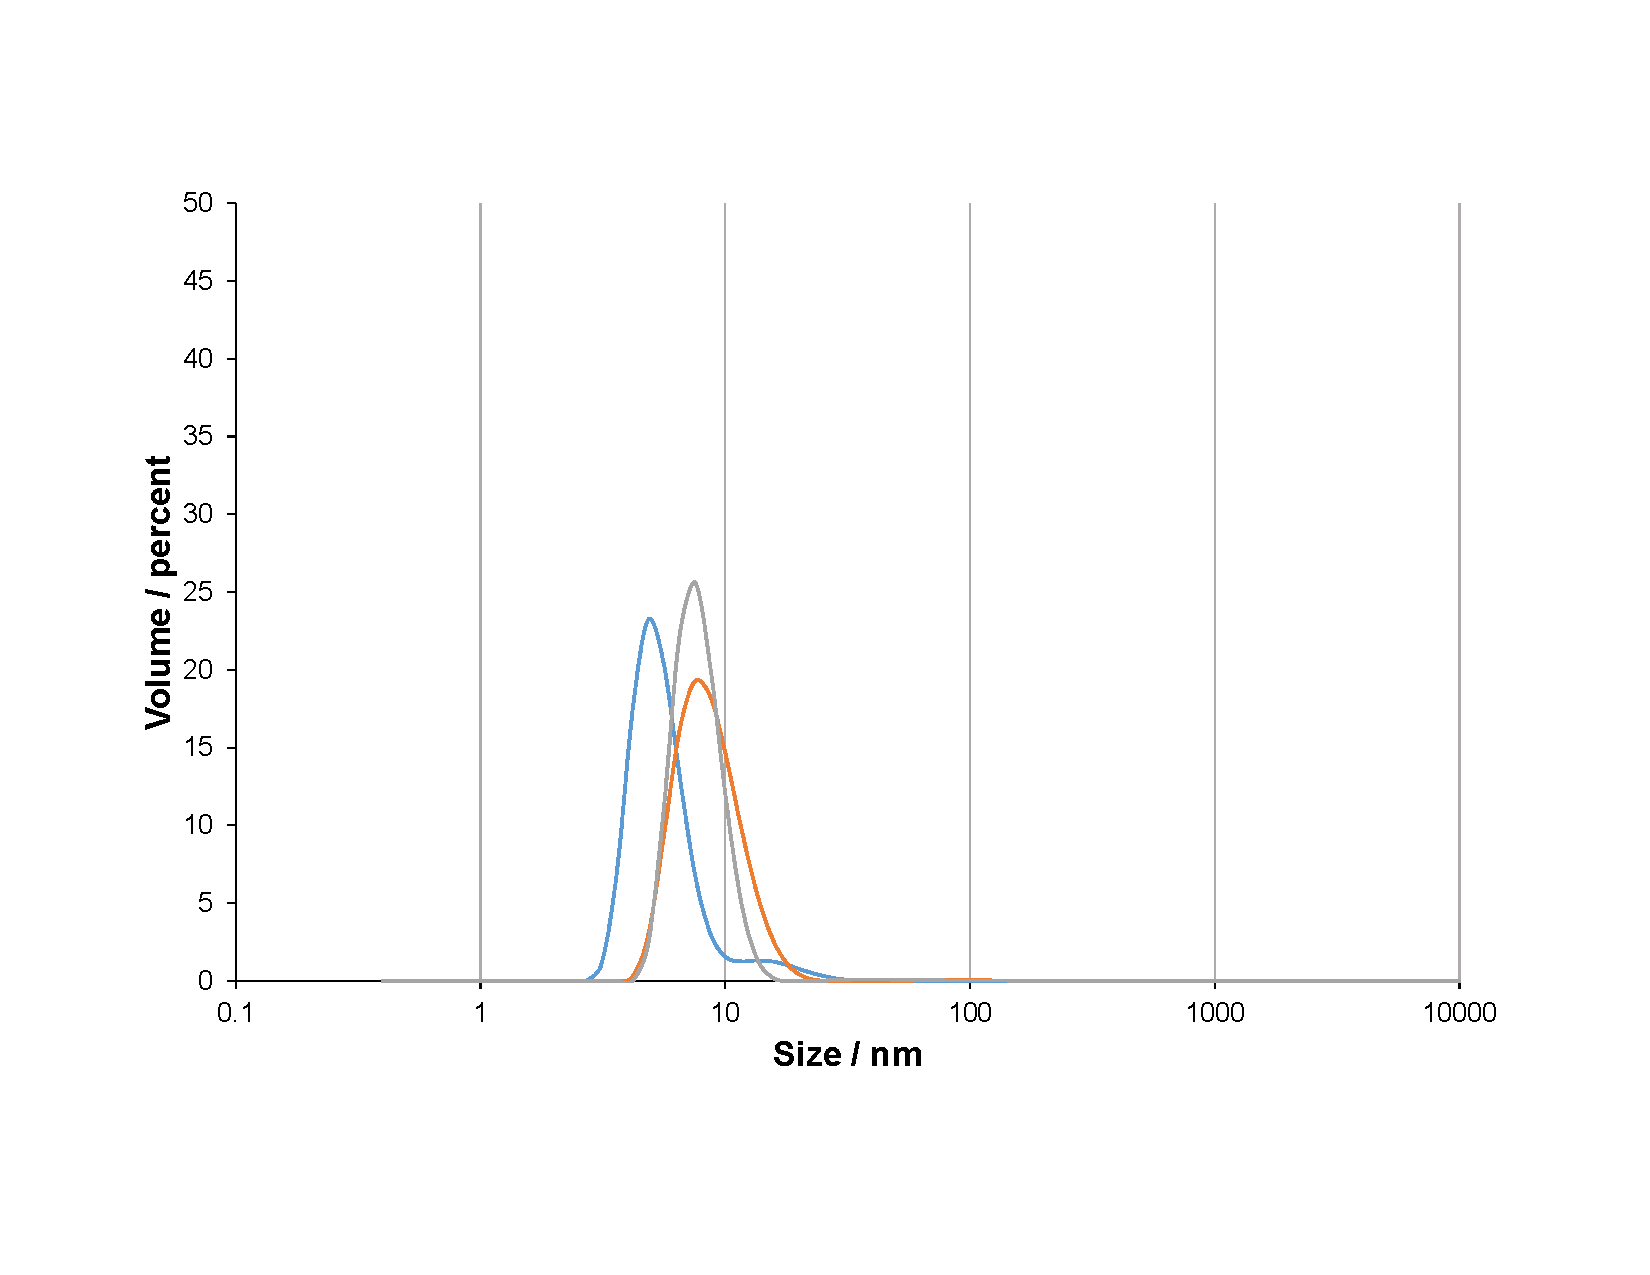
\includegraphics[scale=0.47]{DLS/KAT1_19_0_25mg_ml-1_volume.pdf}
\caption{Volume distribution of a 0.25 mg ml\textsuperscript{-1} sample of C\textsubscript{16}-L-Ala-L-Lys}
\label{volume_0.25_KAT1.19}
\end{figure}

\begin{figure} [ht!]
\centering
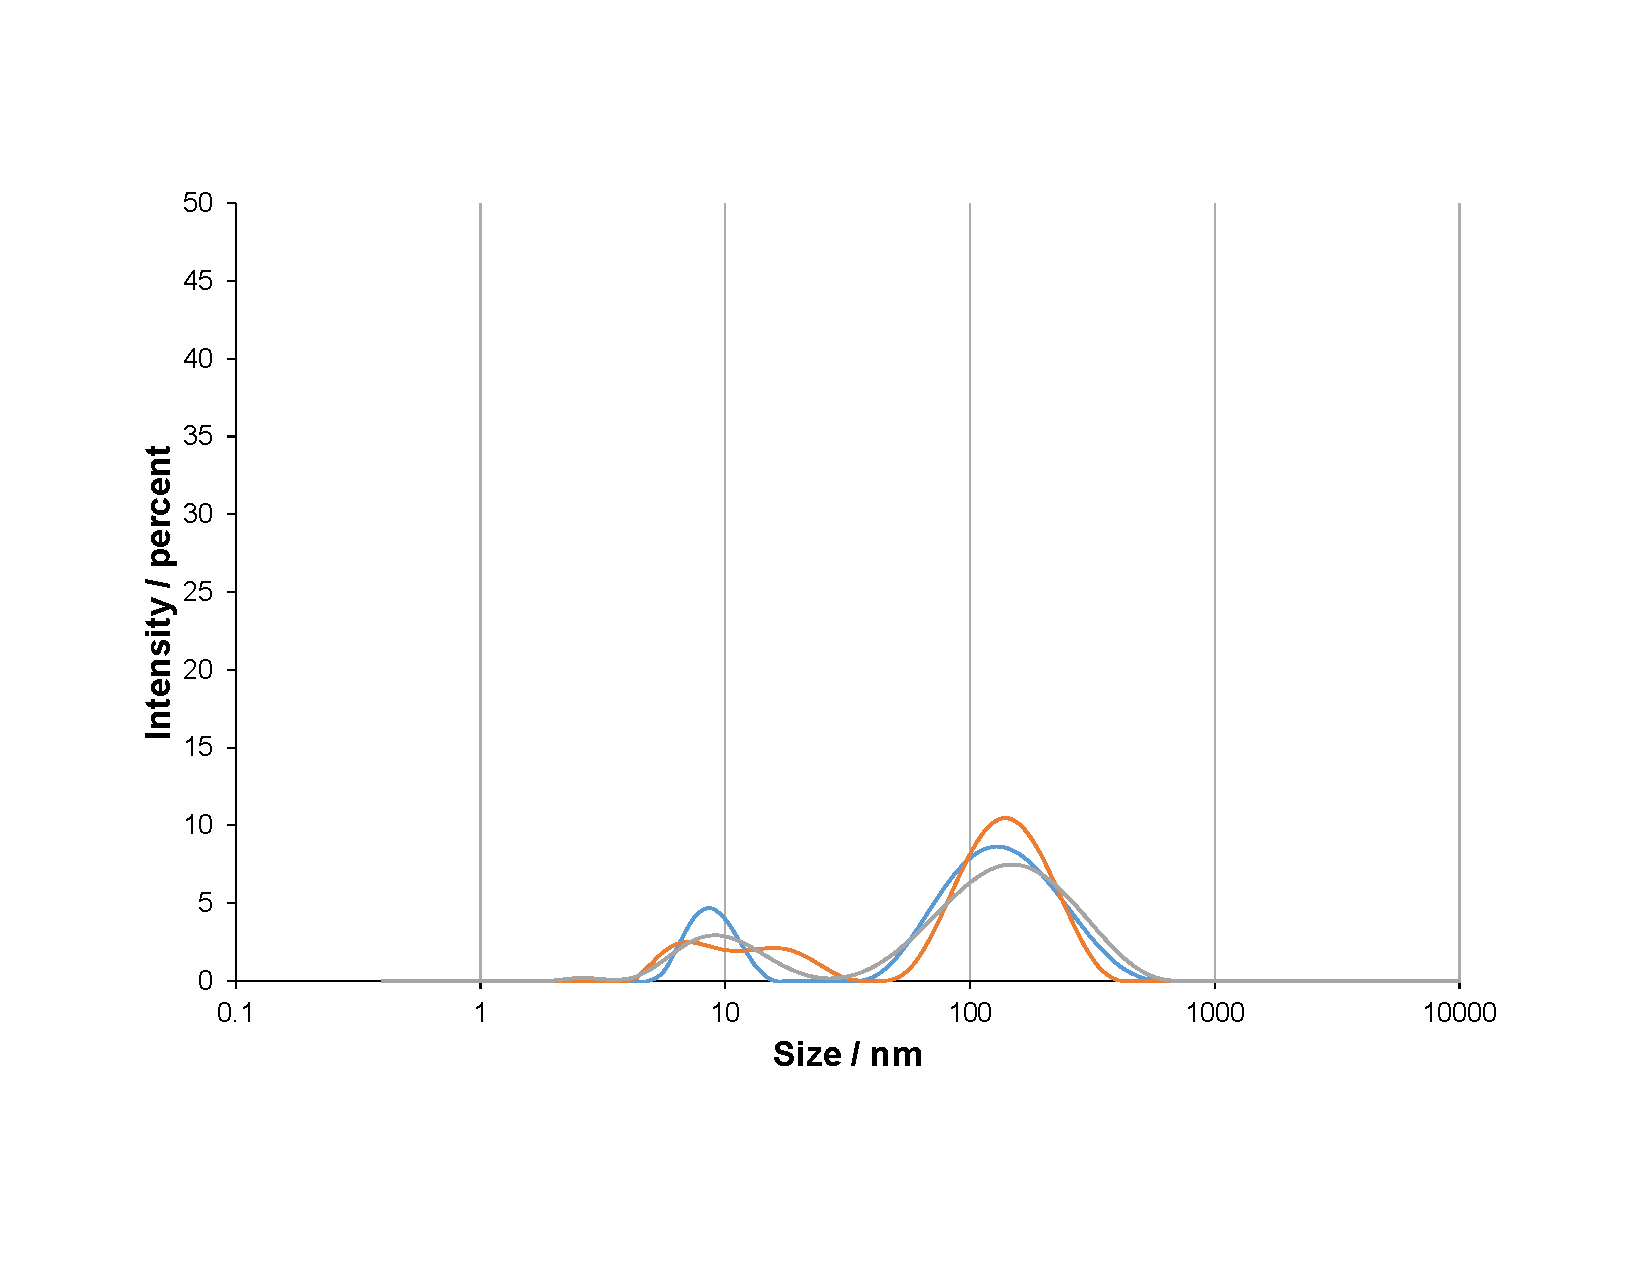
\includegraphics[scale=0.47]{DLS/KAT1_19_1_0mg_ml-1_size.pdf}
\caption{Intensity distribution of a 1 mg ml\textsuperscript{-1} sample of C\textsubscript{16}-L-Ala-L-Lys}
\label{intensity_distribution_KAT1.19}
\end{figure}

\begin{figure} [ht!]
\centering
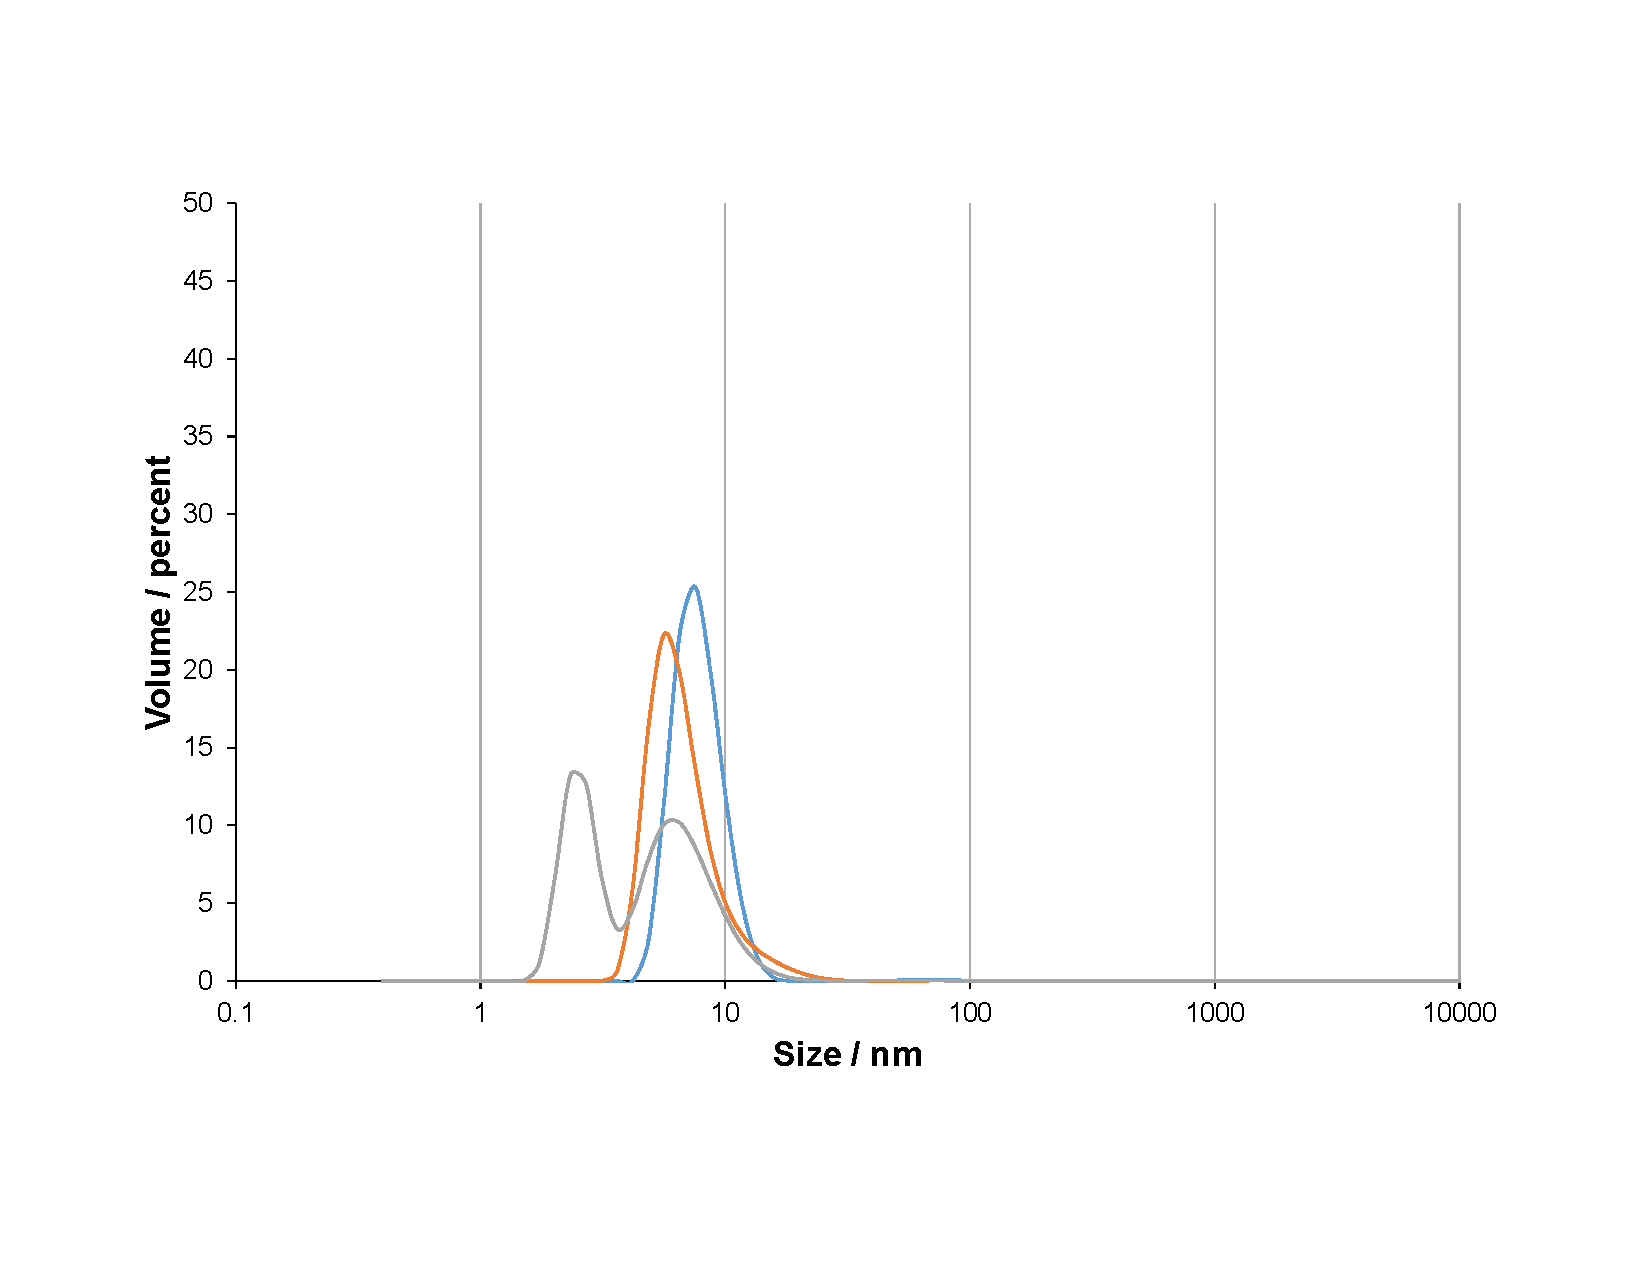
\includegraphics[scale=0.47]{DLS/KAT1_19_1_0mg_ml-1_volume.pdf}
\caption{Volume distribution of a 1 mg ml\textsuperscript{-1} sample of C\textsubscript{16}-L-Ala-L-Lys}
\label{volume_distribution_KAT1.19}
\end{figure}

\begin{figure} [ht!]
\centering
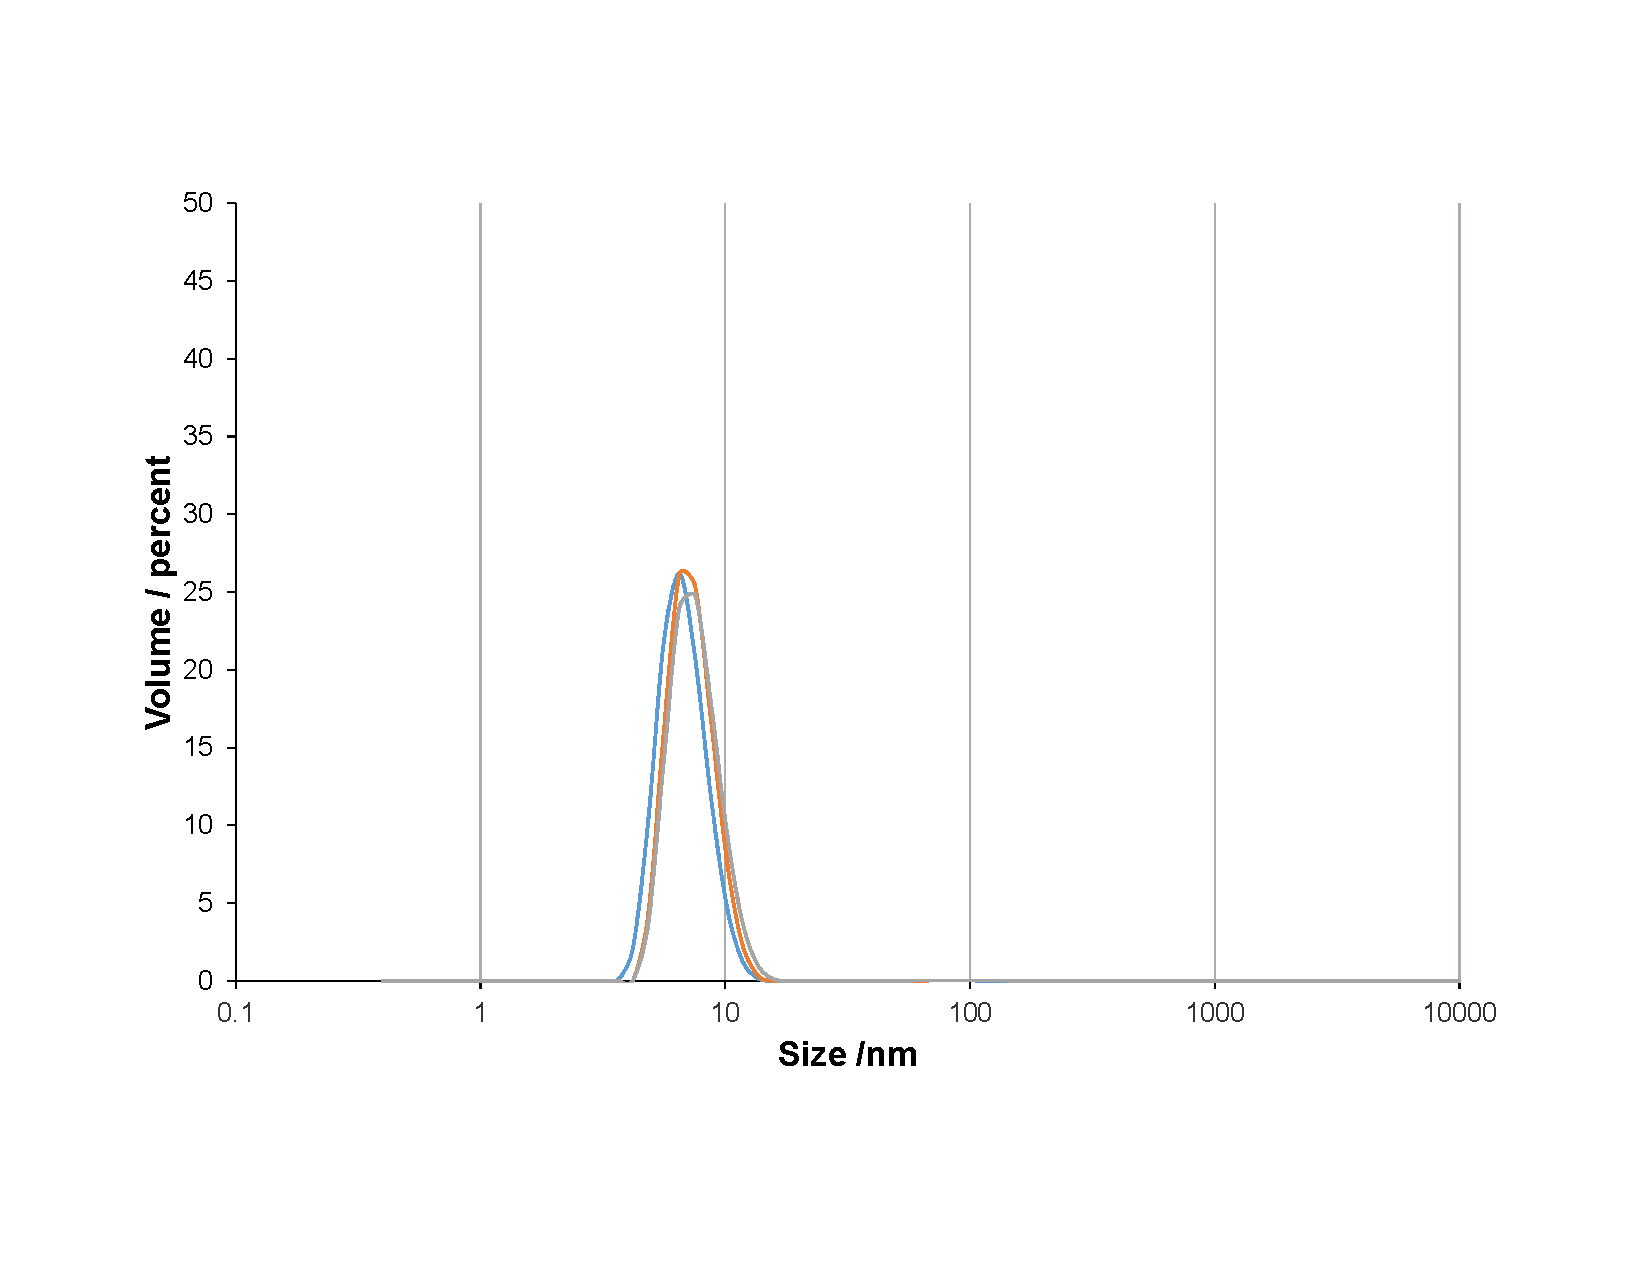
\includegraphics[scale=0.47]{DLS/KAT1_35_1_0mg_ml-1_volume.pdf}
\caption{Volume distribution of a 1 mg ml\textsuperscript{-1} sample of C\textsubscript{16}-D-Ala-D-Lys}
\label{volume_1.0_KAT1.35}
\end{figure}

\begin{figure} [ht!]
\centering
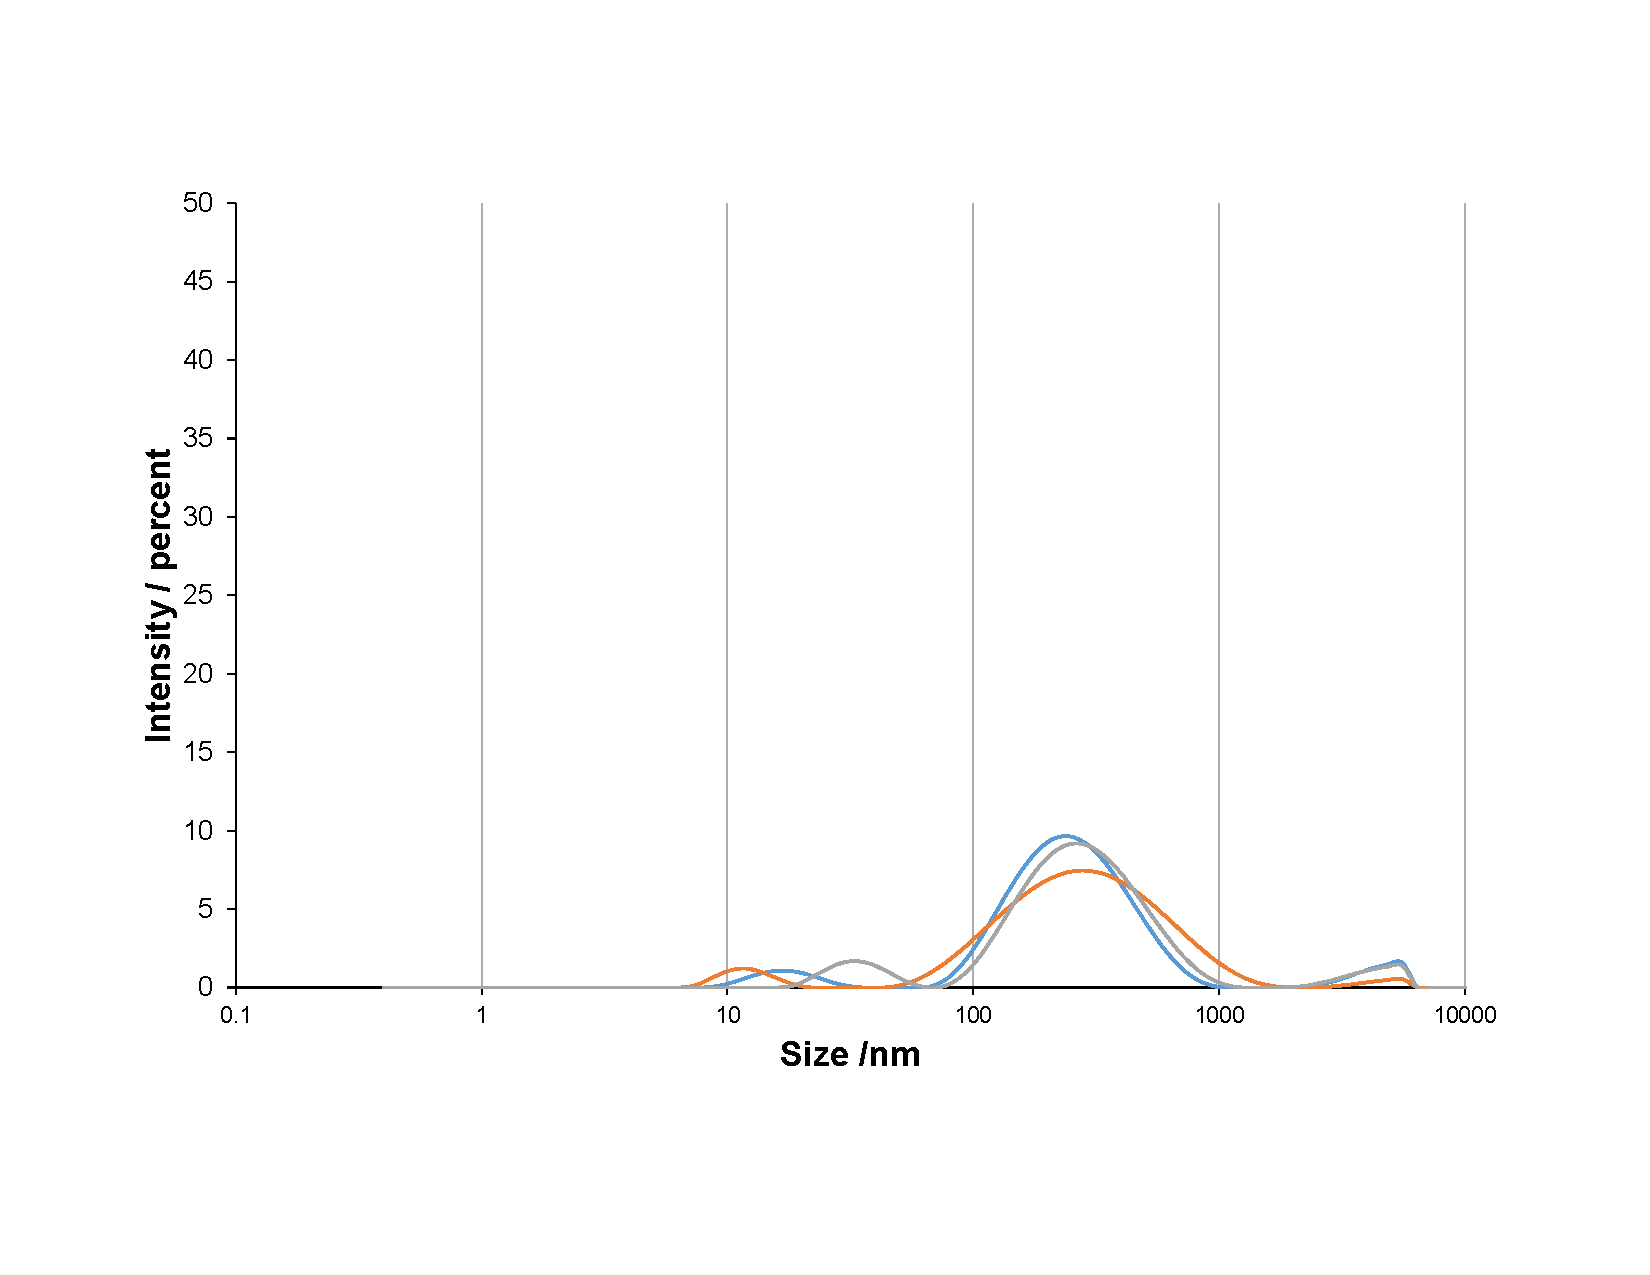
\includegraphics[scale=0.47]{DLS/KAT1_30_1_0mg_ml-1_size.pdf}
\caption{Intensity distribution of a 1.0 mg ml\textsuperscript{-1} sample of C\textsubscript{16}-L-Ala-D-Lys}
\label{size_distribution_KAT1.30_1.0}
\end{figure}
\begin{figure} [ht!]
\centering
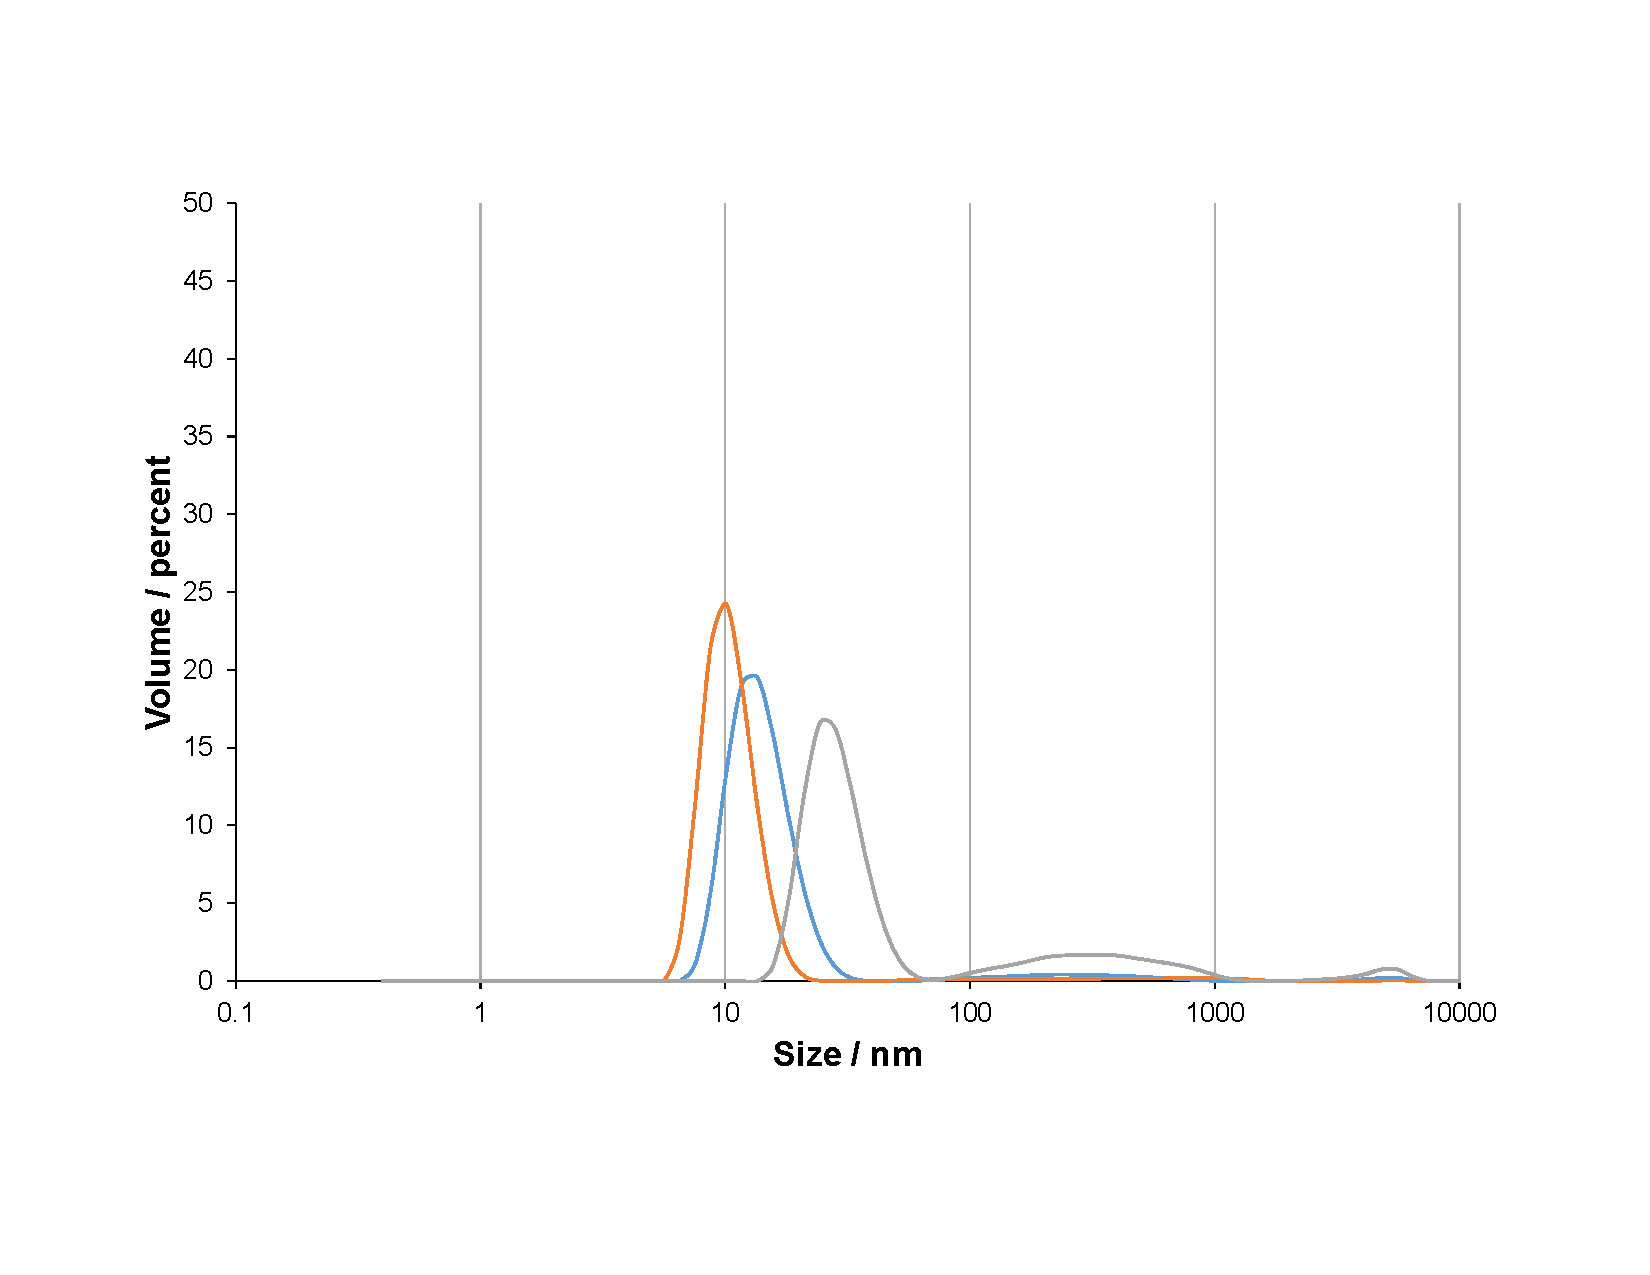
\includegraphics[scale=0.47]{DLS/KAT1_30_1_0mg_ml-1_volume.pdf}
\caption{Volume distribution of a 1.0 mg ml\textsuperscript{-1} sample of C\textsubscript{16}-L-Ala-D-Lys}
\label{volume_distribution_KAT1.30_1.0}
\end{figure}

\begin{figure} [ht!]
\centering
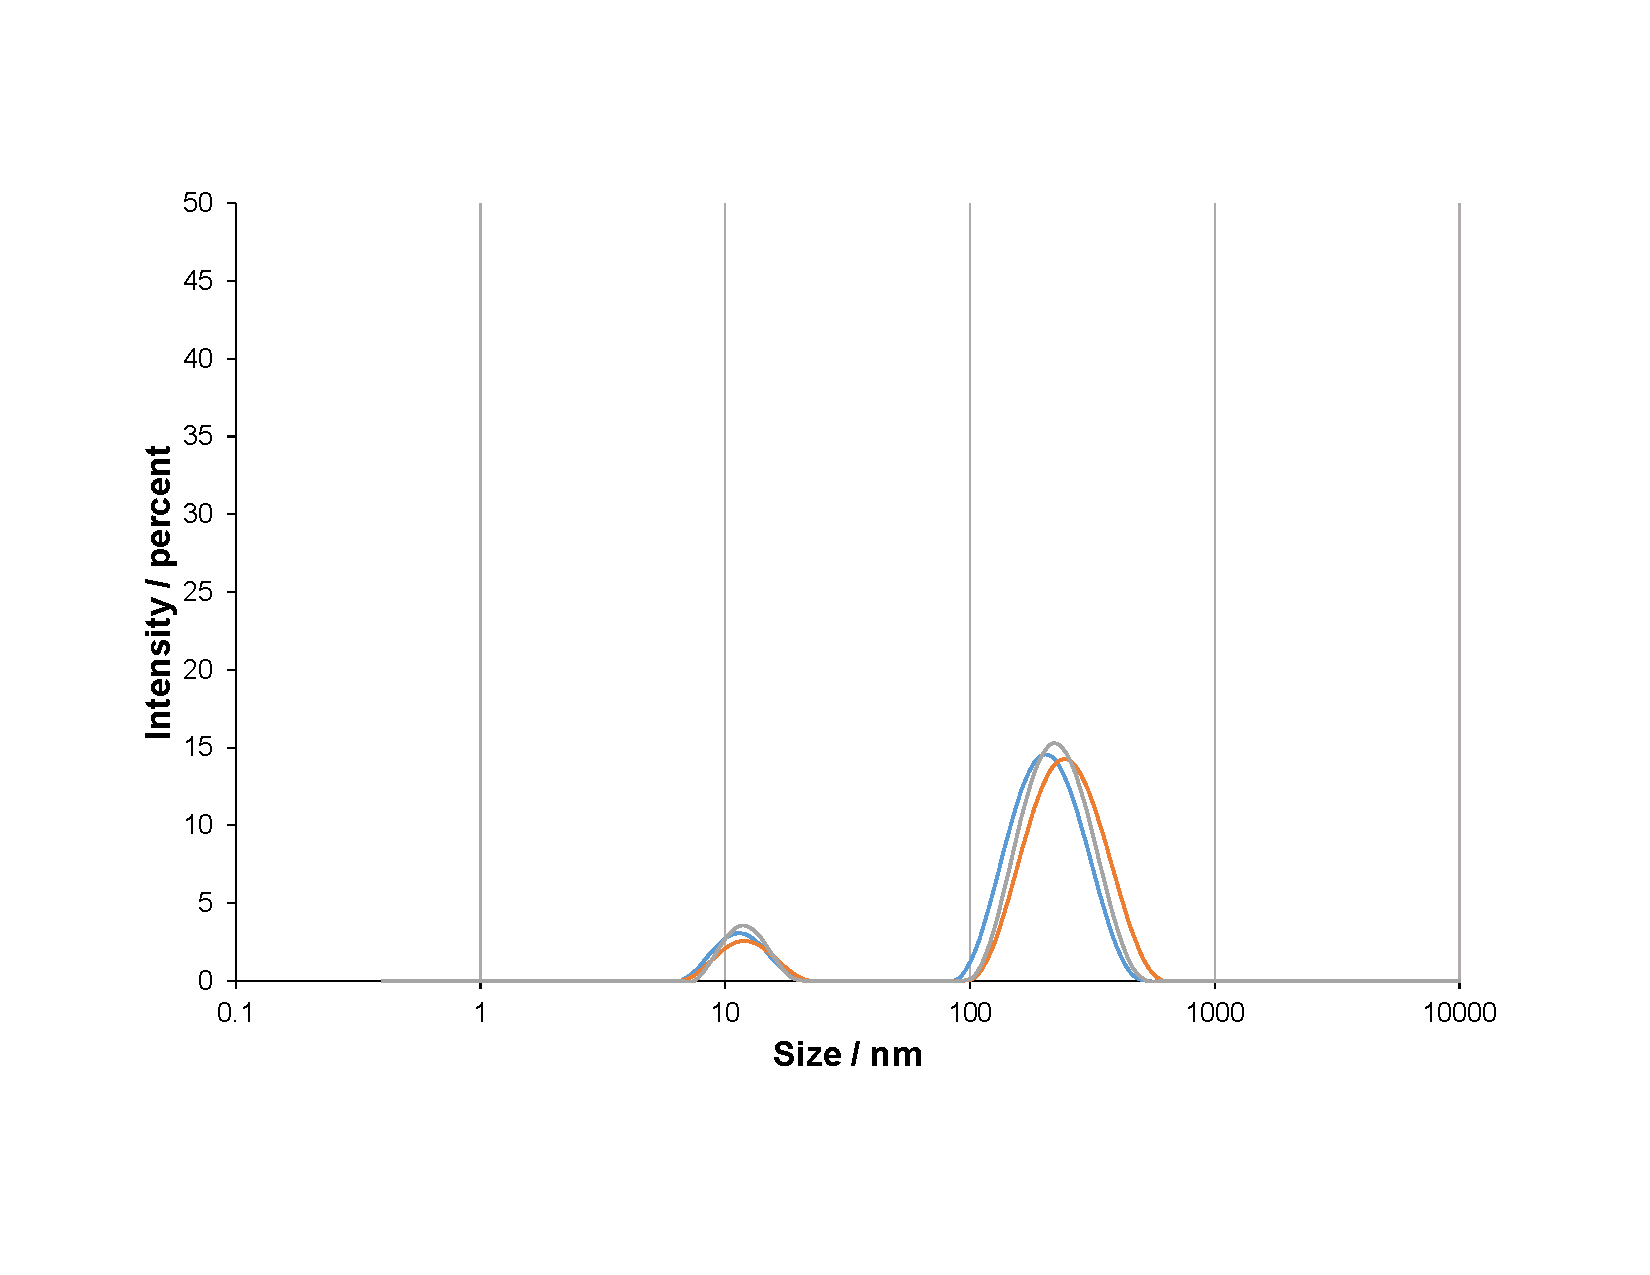
\includegraphics[scale=0.47]{DLS/KAT1_30_0_25mg_ml-1_size.pdf}
\caption{Intensity distribution of a 0.25 mg ml\textsuperscript{-1} sample of C\textsubscript{16}-L-Ala-D-Lys}
\label{intensity_distribution_KAT1.30_0.25}
\end{figure}
\begin{figure} [ht!]
\centering
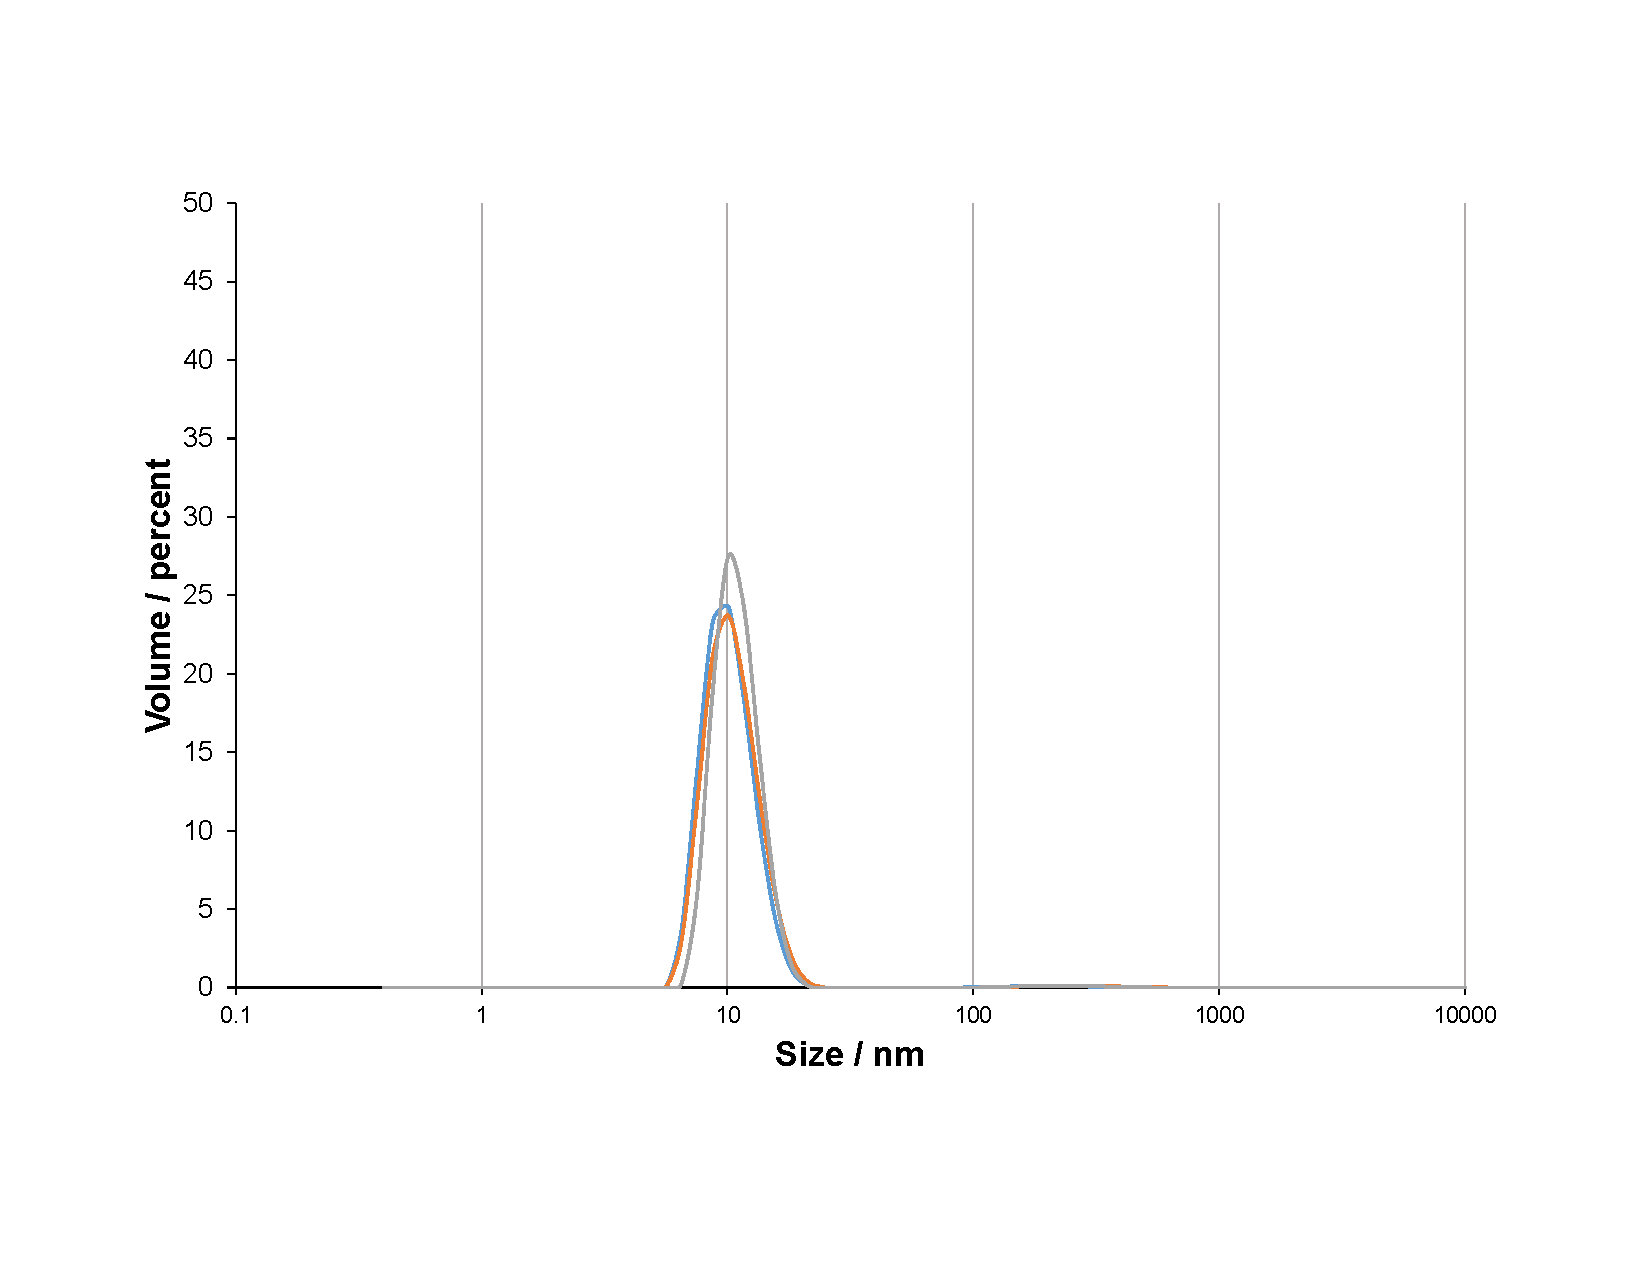
\includegraphics[scale=0.47]{DLS/KAT1_30_0_25mg_ml-1_volume.pdf}
\caption{Volume distribution of a 0.25 mg ml\textsuperscript{-1} sample of C\textsubscript{16}-L-Ala-D-Lys}
\label{Volume_distribution_KAT1.30_0.25}
\end{figure}

\newpage
\begin{figure} [ht!]
\centering
 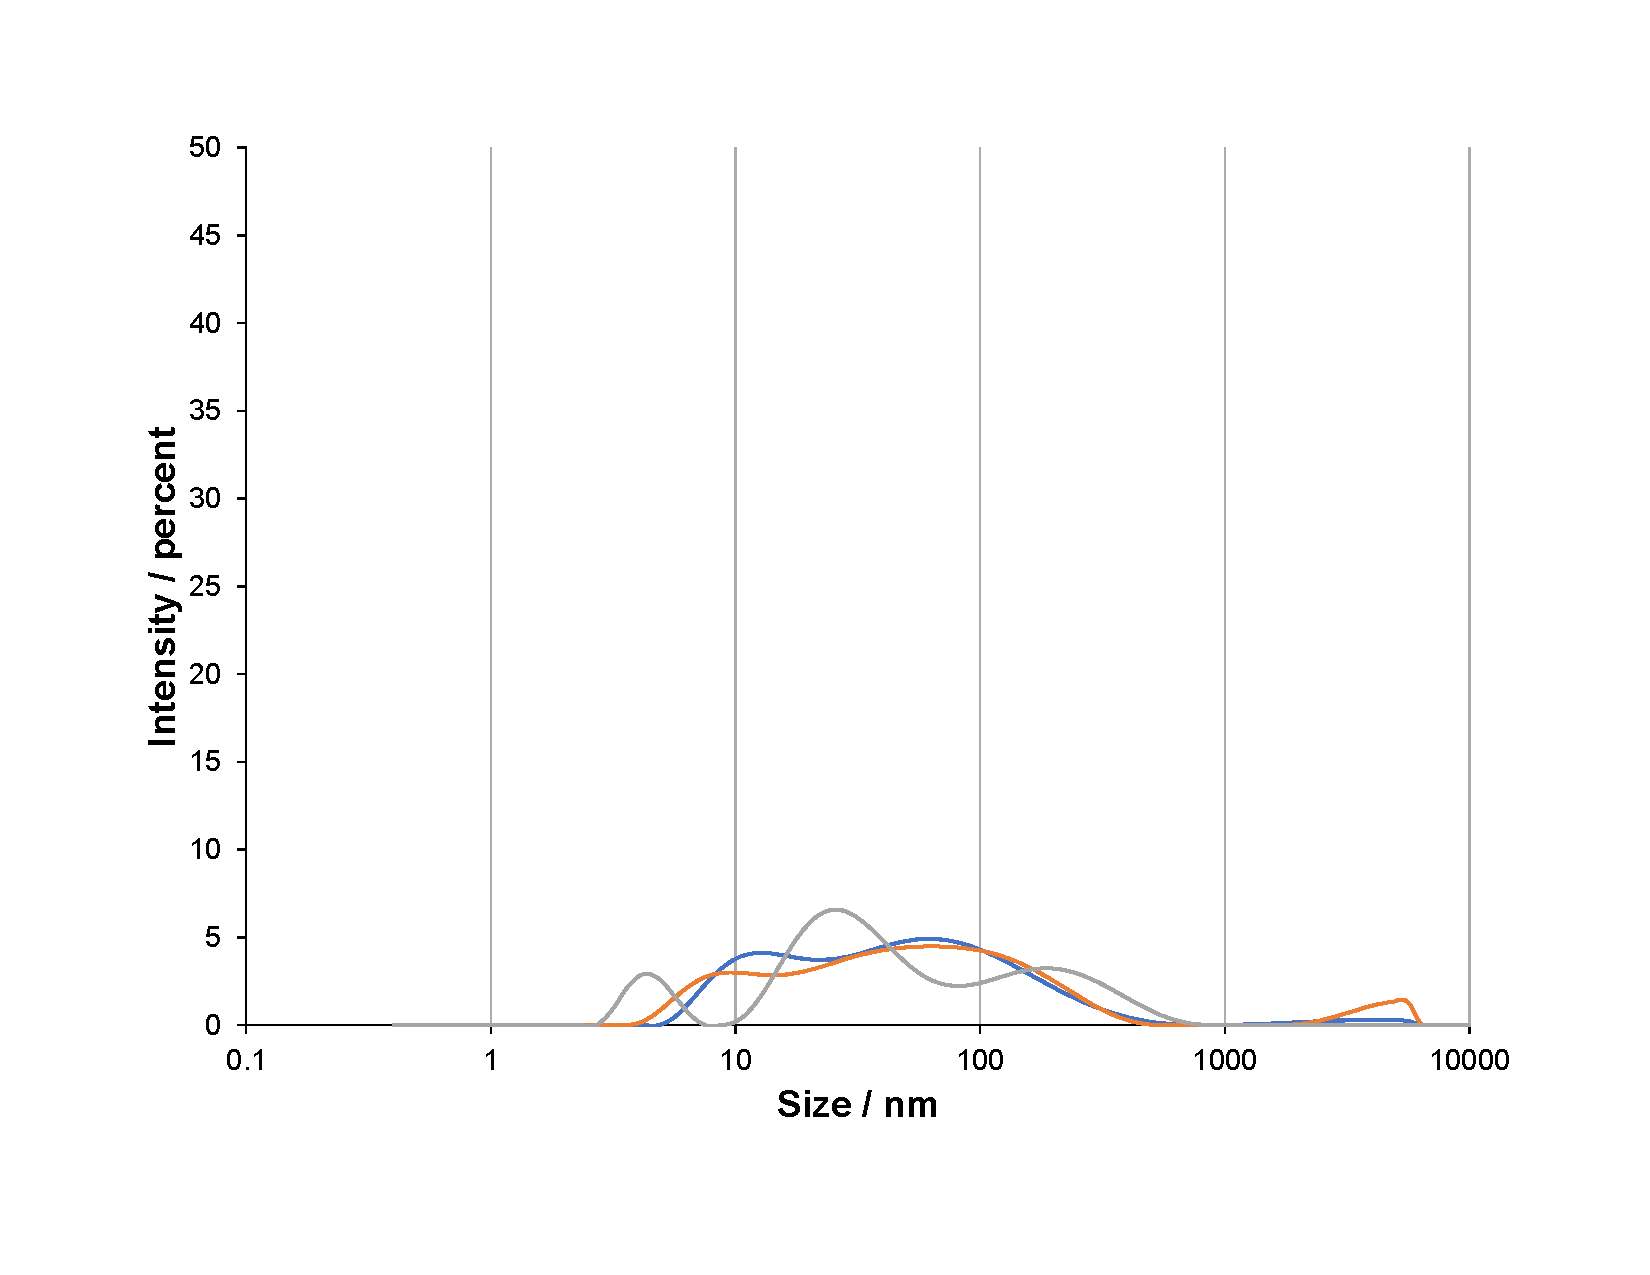
\includegraphics[scale=0.47]{DLS/KAT1_22_0_25mg_ml-1_size.pdf}
\caption{Intensity distribution of a 0.25 mg ml\textsuperscript{-1} sample of C\textsubscript{16}-D-Ala-L-Lys}
\label{intensity_distribution_KAT1.22_0.25}
\end{figure}
\begin{figure} [ht!]
\centering
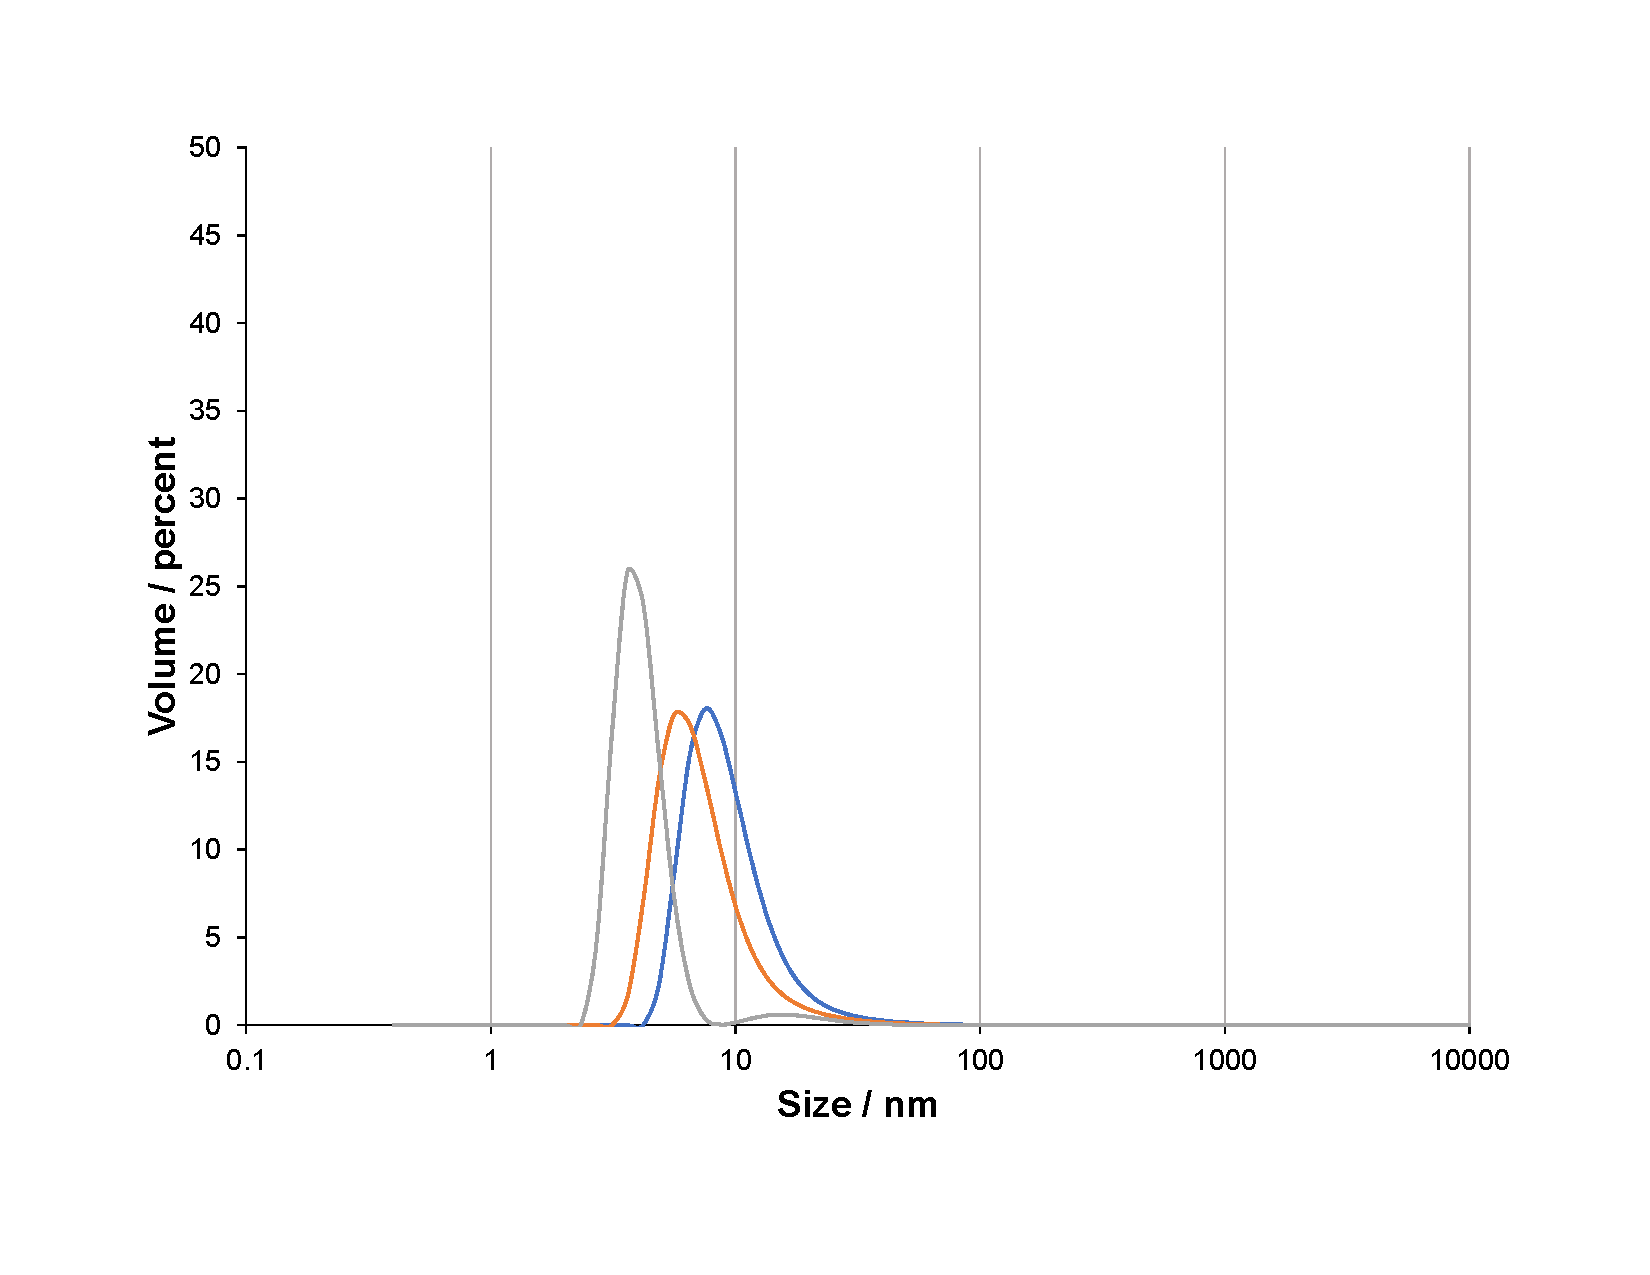
\includegraphics[scale=0.47]{DLS/KAT1_22_0_25mg_ml-1_volume.pdf}
\caption{Volume distribution of a 0.25 mg ml\textsuperscript{-1} sample of C\textsubscript{16}-D-Ala-L-Lys}
\label{volume_distribution_KAT1.22_0.25}
\end{figure}
\newpage
\begin{figure} [ht!]
\centering
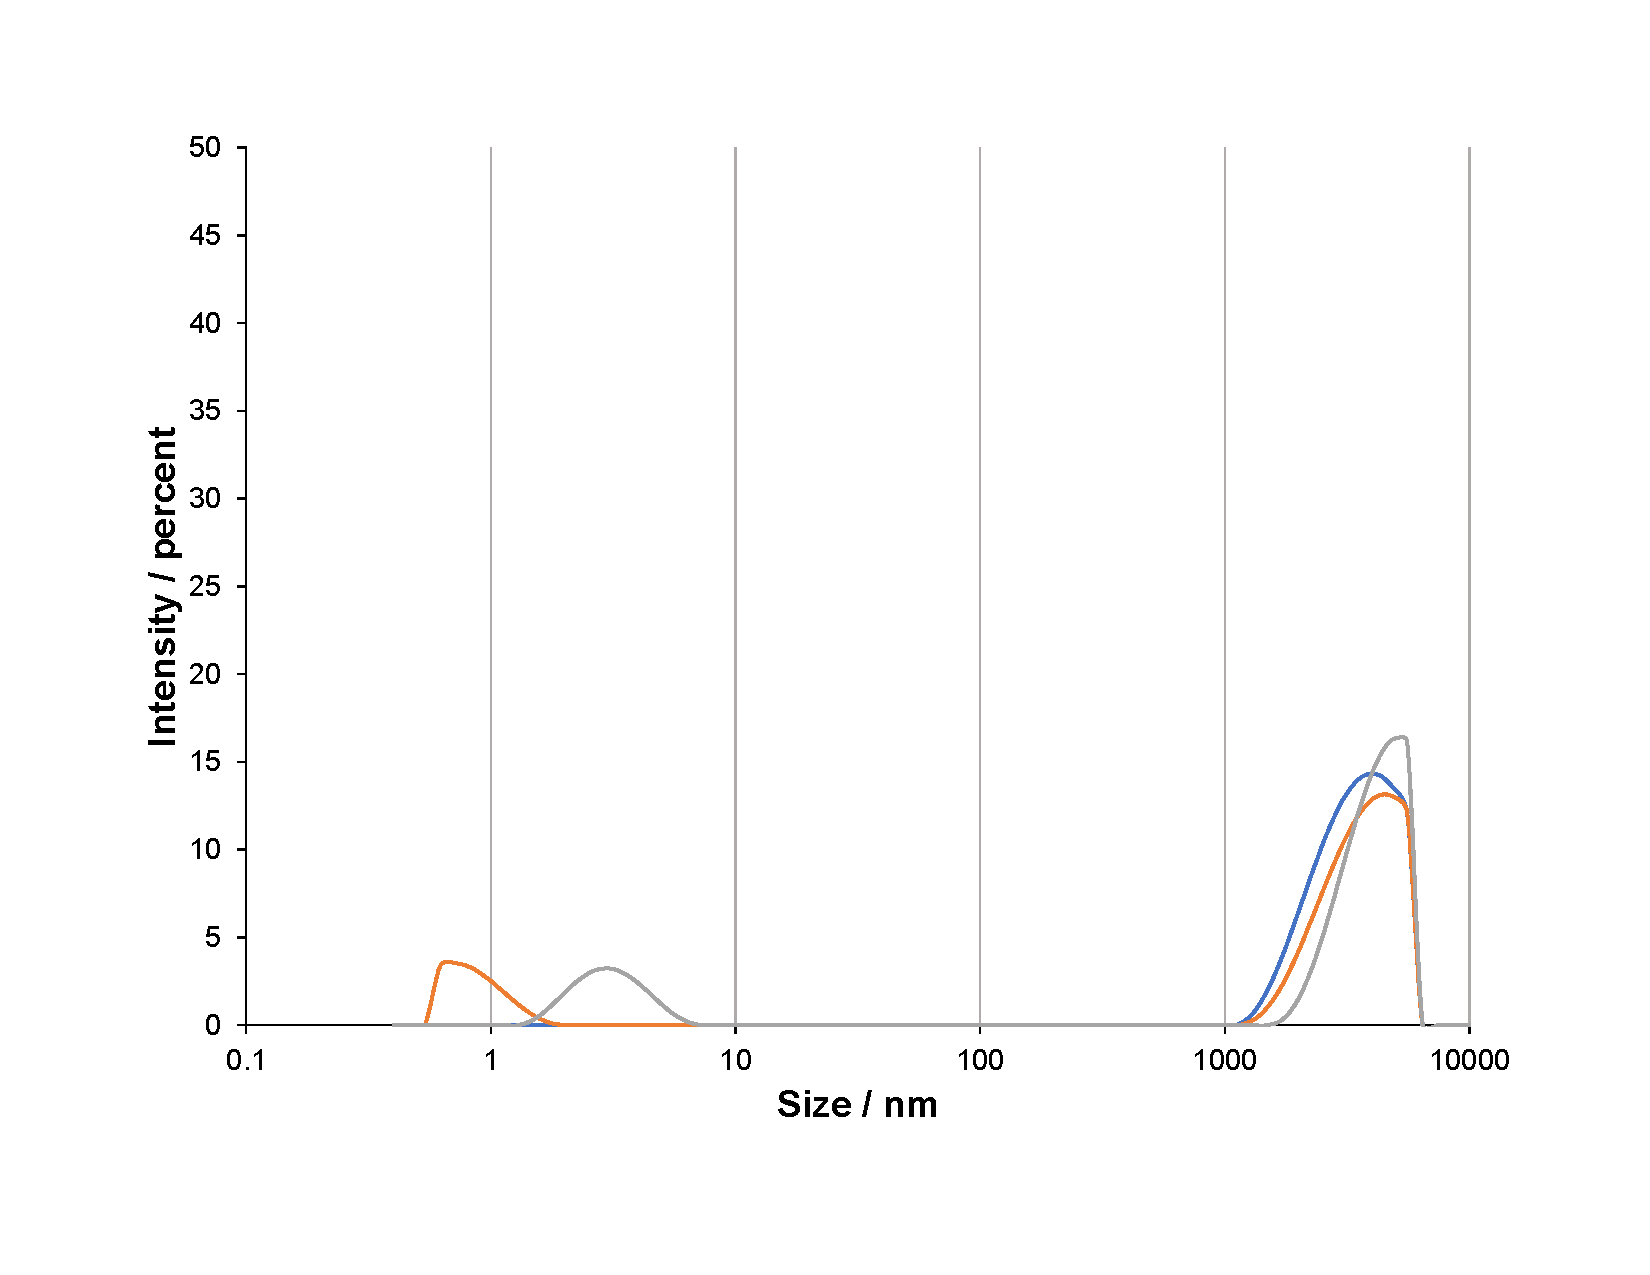
\includegraphics[scale=0.47]{DLS/KAT1_22_1_0mg_ml-1_size.pdf}
\caption{Intensity distribution of a 1 mg ml\textsuperscript{-1} sample of C\textsubscript{16}-D-Ala-L-Lys}
\label{intensity_distribution_KAT1.22}
\end{figure}
\begin{figure} [ht!]
\centering
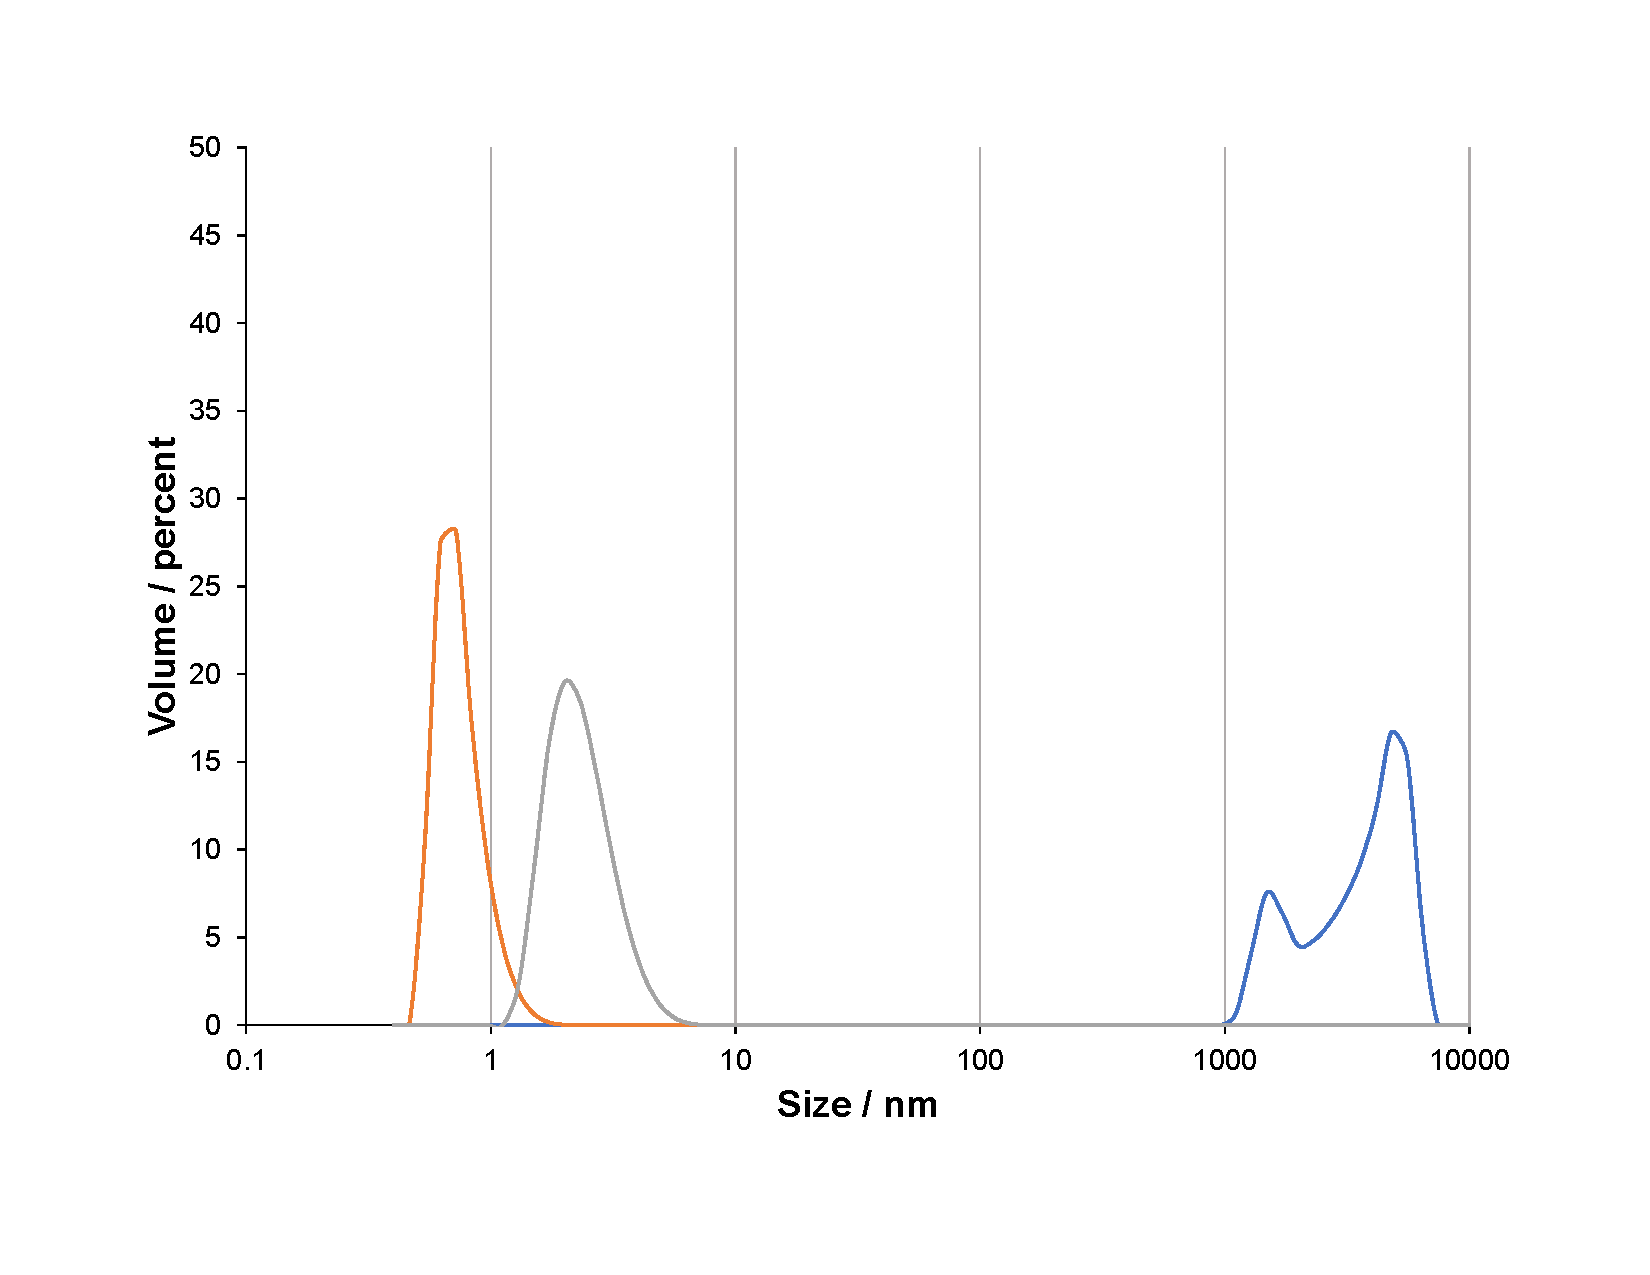
\includegraphics[scale=0.47]{DLS/KAT1_22_1_0mg_ml-1_volume.pdf}
\caption{Volume distribution of a 1 mg ml\textsuperscript{-1} sample of C\textsubscript{16}-D-Ala-L-Lys}
\label{volume_distribution_KAT1.22}
\end{figure}

\begin{table}[ht!]
\caption{A summary of the data obtained by DLS for each compound.}
\begin{tabular}{l|l|l}
\textbf{Compound name} & \textbf{Concentration / mg ml\textsuperscript{-1}} & \textbf{Z-Average / nm}\\
\hline
\textbf{C\textsubscript{16}-L-Ala-L-Lys} & 0.25 & 63.66 $\pm$ 1.56  \\

\textbf{C\textsubscript{16}-L-Ala-L-Lys} & 1.0 & 53.25 $\pm$ 1.10  \\

\textbf{C\textsubscript{16}-D-Ala-D-Lys} & 0.25  & 66.52 $\pm$ 1.03\\

\textbf{C\textsubscript{16}-D-Ala-D-Lys} & 1.0  & 52.90 $\pm$ 1.12\\

\textbf{C\textsubscript{16}-L-Ala-D-Lys} & 0.25 & 100 $\pm$ 13.78 \\

\textbf{C\textsubscript{16}-L-Ala-D-Lys} & 1.0 & 179.5 $\pm$ 4.79 \\

\textbf{C\textsubscript{16}-D-Ala-L-Lys} & 0.25 & 29.97 $\pm$ 1.70 \\

\textbf{C\textsubscript{16}-D-Ala-L-Lys} & 1.0 & 7912 $\pm$ 1815 \footnotetext{Number average is so high in this case, due to the presence of dust within the cuvette itself}
\\

\end{tabular}
\label{DLS_summary2}
\end{table}
